\documentclass{article}
\usepackage[utf8]{inputenc}
\usepackage{subcaption}
\usepackage{pgfplots}
\pgfplotsset{compat=1.16} % Needed for compatibility reasons and to hide an error
% \usetikzlibrary{external} \tikzexternalize  % Uncomment for making separate pdfs for each figure
 
\title{Quasi-Cooperator }
\author{Colin Cleveland}
\date{\today}

\overfullrule=1mm
\usepackage{xcolor}
% Seaborn 'colorblind' colours -------------------------
\definecolor{C0}{HTML}{cb4335}
\definecolor{C1}{HTML}{2874a6}
\definecolor{C2}{HTML}{fa8072}
\definecolor{C3}{HTML}{85c1e9}
\definecolor{C4}{HTML}{cc78bc}
\definecolor{C5}{HTML}{ca9161}
\definecolor{C6}{HTML}{fbafe4}
\definecolor{C7}{HTML}{949494}
\definecolor{C8}{HTML}{ece133}
\definecolor{C9}{HTML}{56b4e9}
\pgfplotscreateplotcyclelist{colorblind}{%
    {C0,fill=C0,fill opacity=.8,mark=C0},
    {C1,fill=C1,fill opacity=.8,mark=C1},
    {C2,fill=C2,fill opacity=.8,mark=C2},
    {C3,fill=C3,fill opacity=.8,mark=C3},
    {C4,fill=C4,fill opacity=.8,mark=C4},
    {C5,fill=C5,fill opacity=.8,mark=C5},
    {C6,fill=C6,fill opacity=.8,mark=C6},
    {C7,fill=C7,fill opacity=.8,mark=C7},
    {C8,fill=C8,fill opacity=.8,mark=C8},
    {C9,fill=C9,fill opacity=.8,mark=C9}
    }
\pgfplotscreateplotcyclelist{colorblind}{
{color = C0,mark=*},
{color = C1,mark=triangle},
{color = C2,mark=o},
{C3,thick,densely dotted},
{color = C4, mark = square},
{C5,thick},
{C6,thick},
{C7,thick},
{C8,thick},
{C9,thick}
}

%------------------------------------------------------


\begin{document}

\maketitle

In the original setting, when $\rho = 0.5,  \delta = 0.1, ,m=0.2$, QC stops being 0 when $b > 1.5$. To make the $\alpha$ and $\lambda$ graph more meaningful, I choose the $b = 1.53$ when $b$ is the fixed parameter.


 \begin{figure}[h!t]
    \centering
    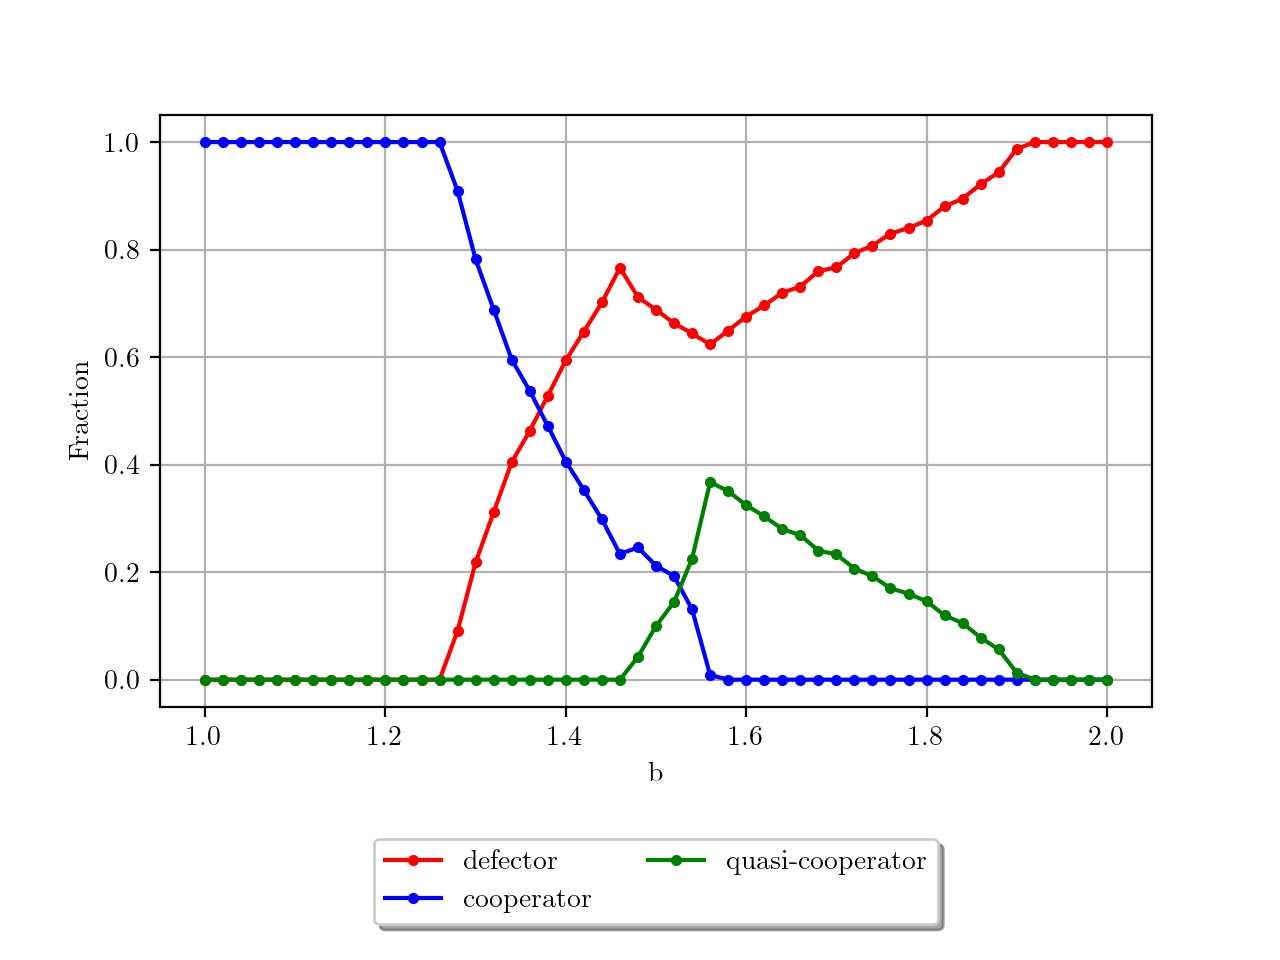
\includegraphics[width=\textwidth]{cg_B_200.png}
    \caption{Parameters: $ \rho = 0.5,\alpha =0.1,  \delta = 0.1, m=0.2, \lambda = 0.7$.}
    \label{fig:b200}
\end{figure}

\clearpage


 \begin{figure}[h!t]
    \centering
    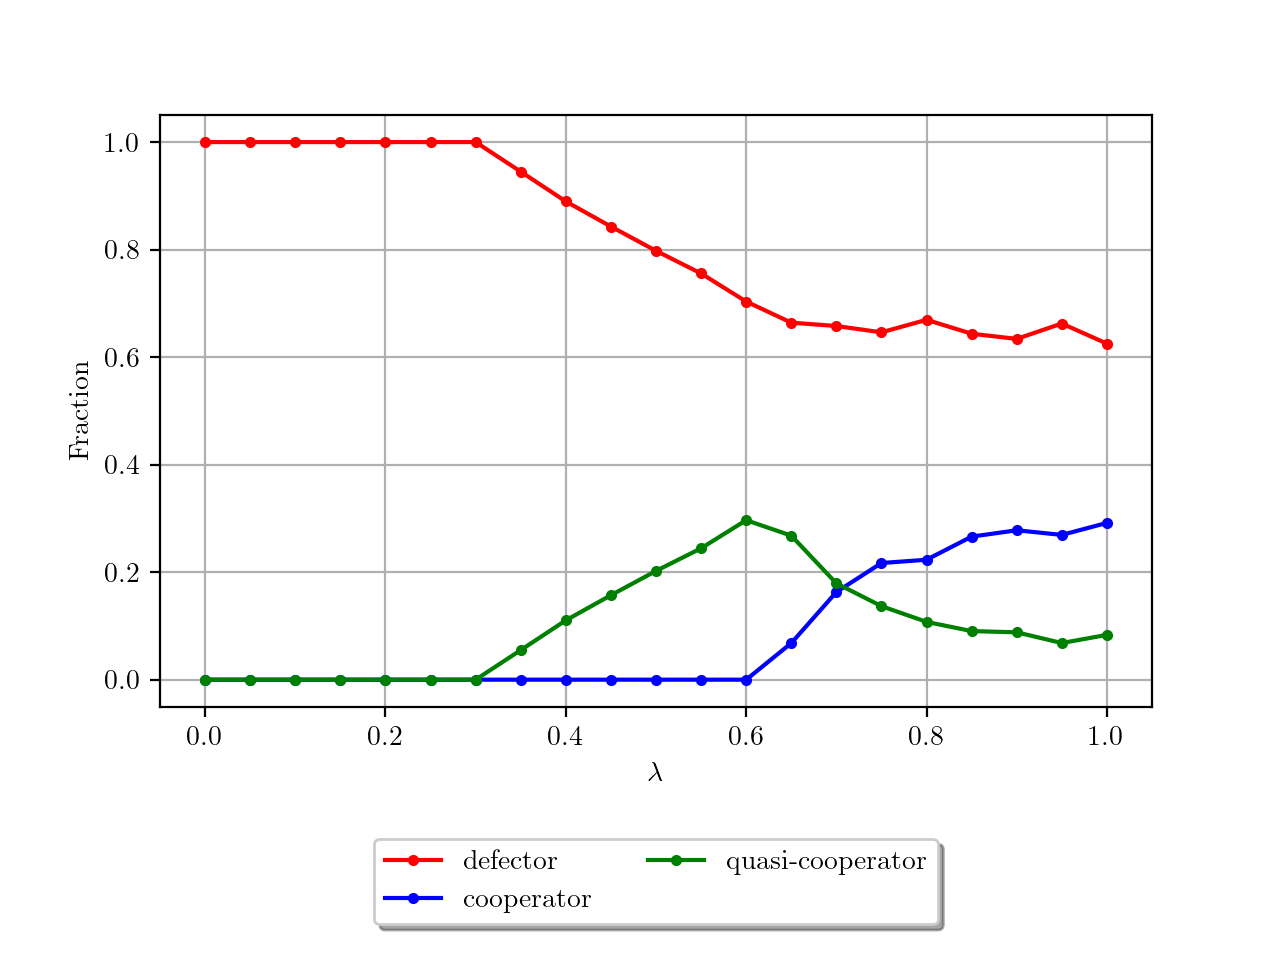
\includegraphics[width=\textwidth]{cg_L_200.png}
    \caption{Parameters: $ \rho = 0.5,\alpha =0.1,  \delta = 0.1, m=0.2, b = 1.53$.}
    \label{fig:lambda200}
\end{figure}

 \begin{figure}[h!t]
    \centering
    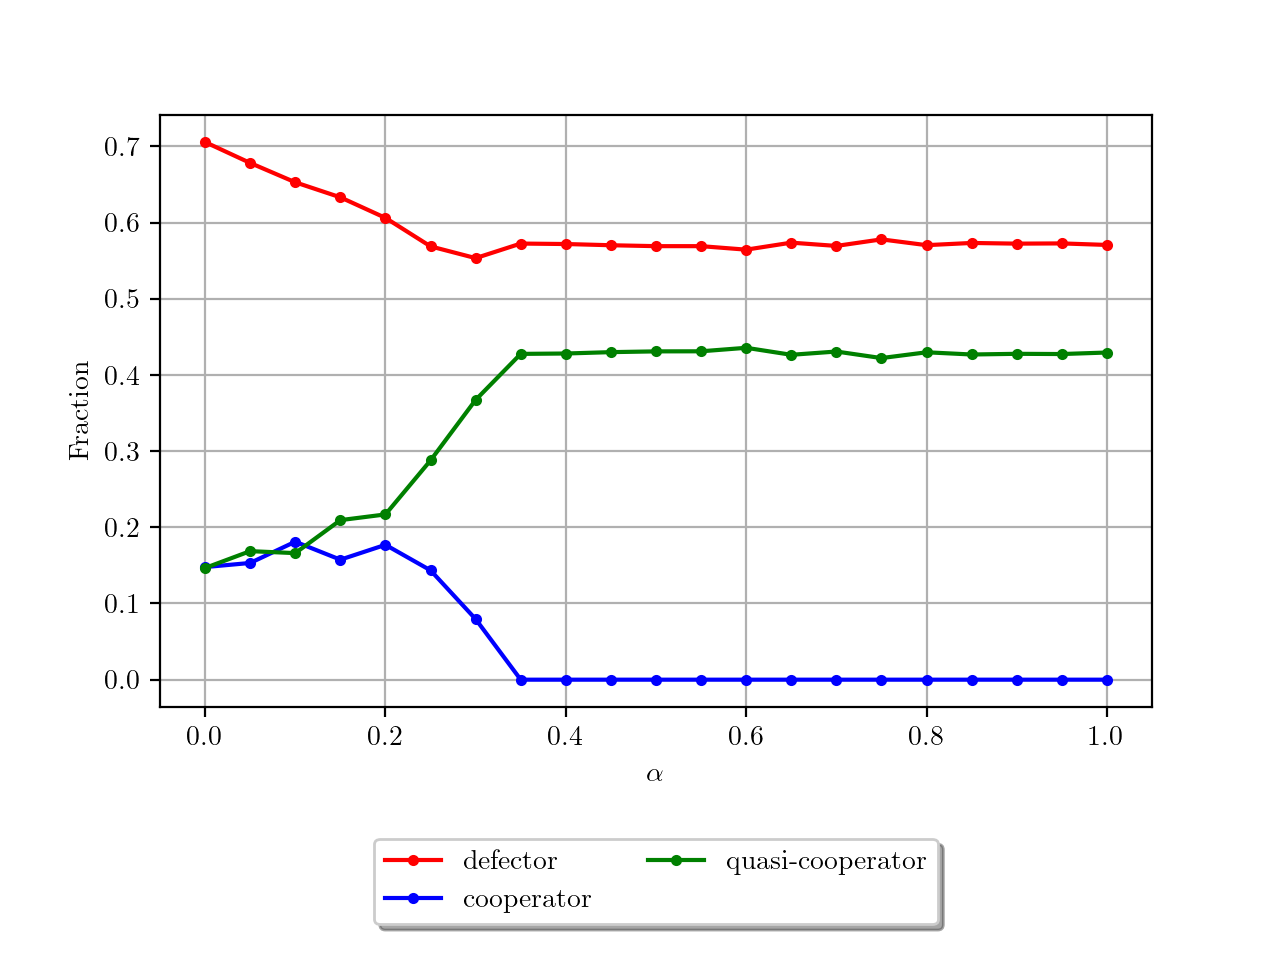
\includegraphics[width=\textwidth]{cg_A_200.png}
    \caption{Parameters: $ \rho = 0.5, b = 1.53,  \delta = 0.1, m=0.2, \lambda = 0.7$..}
    \label{fig:alp200}
\end{figure}



 \begin{figure}[h!t]
    \centering
    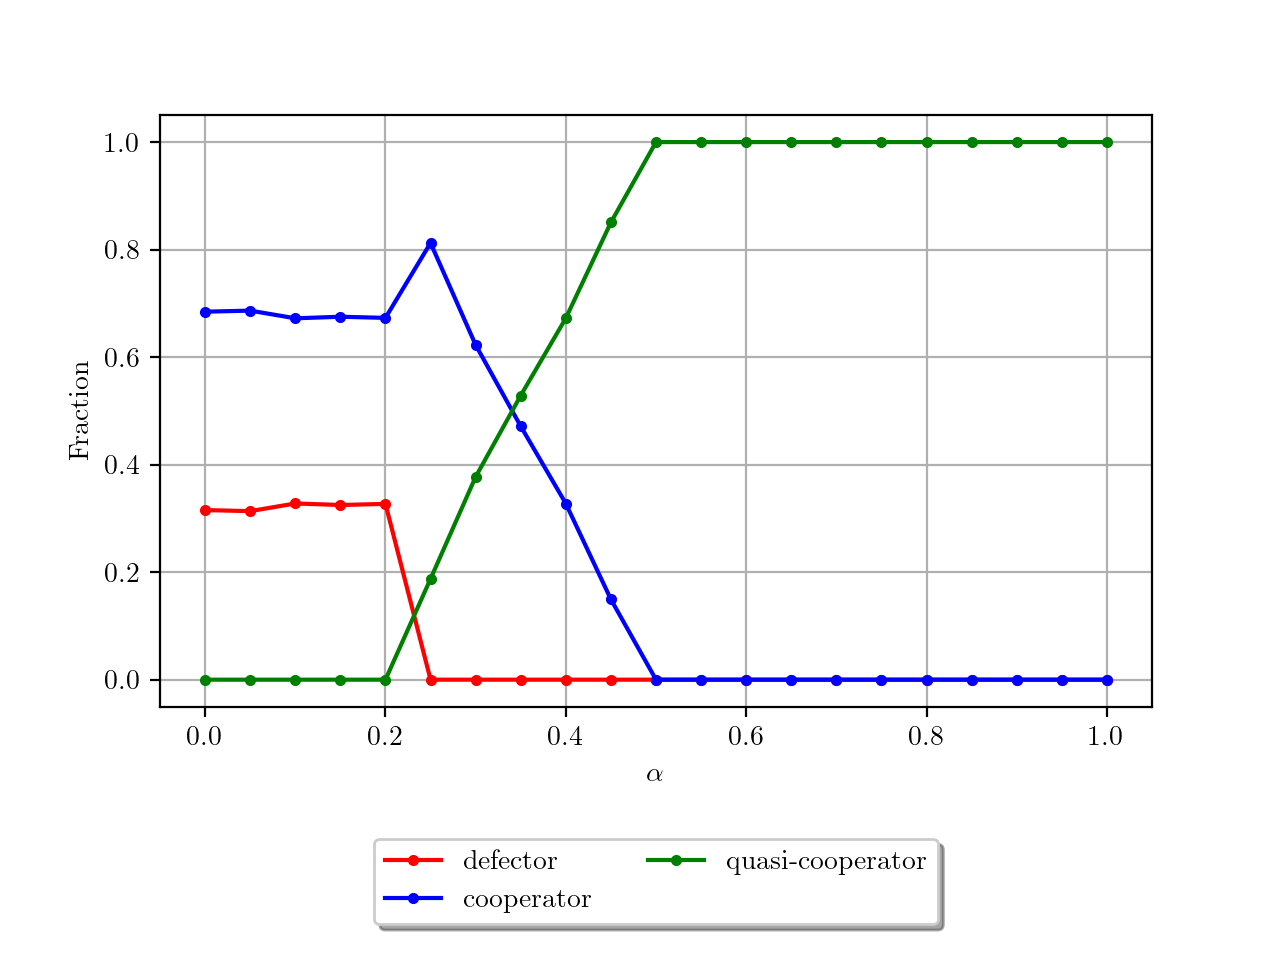
\includegraphics[width=\textwidth]{Low_b.png}
    \caption{Parameters: $ \rho = 0.5, b = 1.32,  \delta = 0.1, m=0.2, \lambda = 0.7$.}
    \label{fig:onlyCs}
\end{figure}

\clearpage

\section{Jan 27th}

To have a general view of how the three kinds of players distributed in different ($\alpha, b,\lambda, m, \delta,\rho$), I use RGB to indicate if a kind of player exist in the simulation as \ref{fig:rgb}. 

\begin{figure}[h]
    \centering
    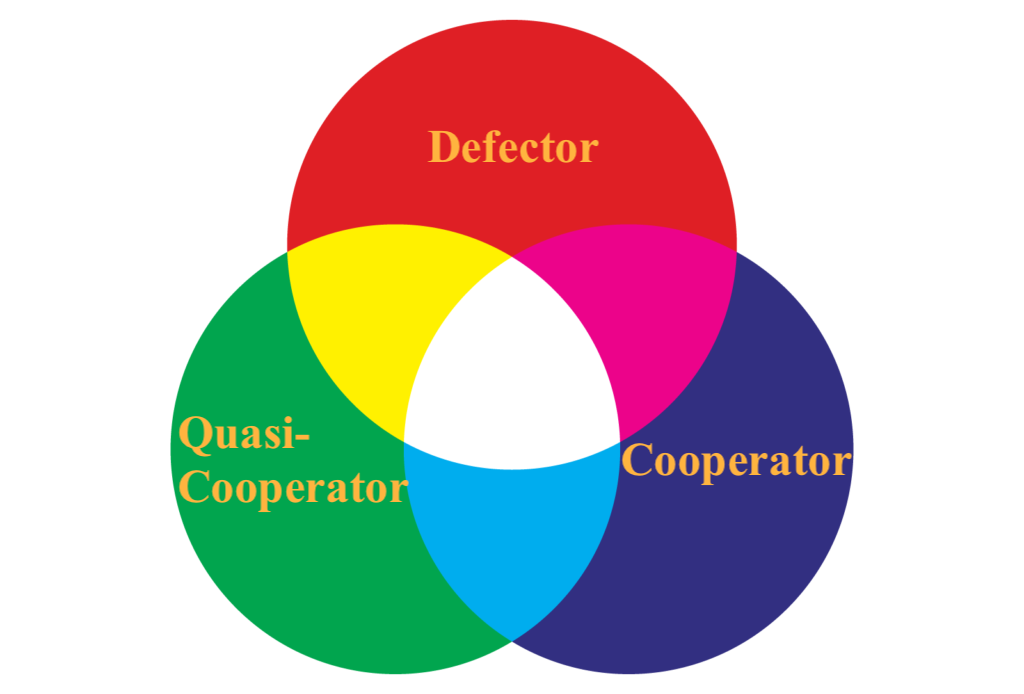
\includegraphics[width=\textwidth]{rgb-color-model-1024x694.png}
    \caption{When there is a defector, we use red to indicated. Similar for Cooperator and Quasi-Cooperator.}
    \label{fig:rgb}
\end{figure}

When we take $\delta = 0.25$ and $\rho = 0.5$, the outcome is roughtly like Fig.\ref{fig:d25r050}. As for the $\delta = 0.1, \rho = 0.5$, it's illustrated in Fig. \ref{fig:d01r05}

\begin{figure}[h]
    \centering
    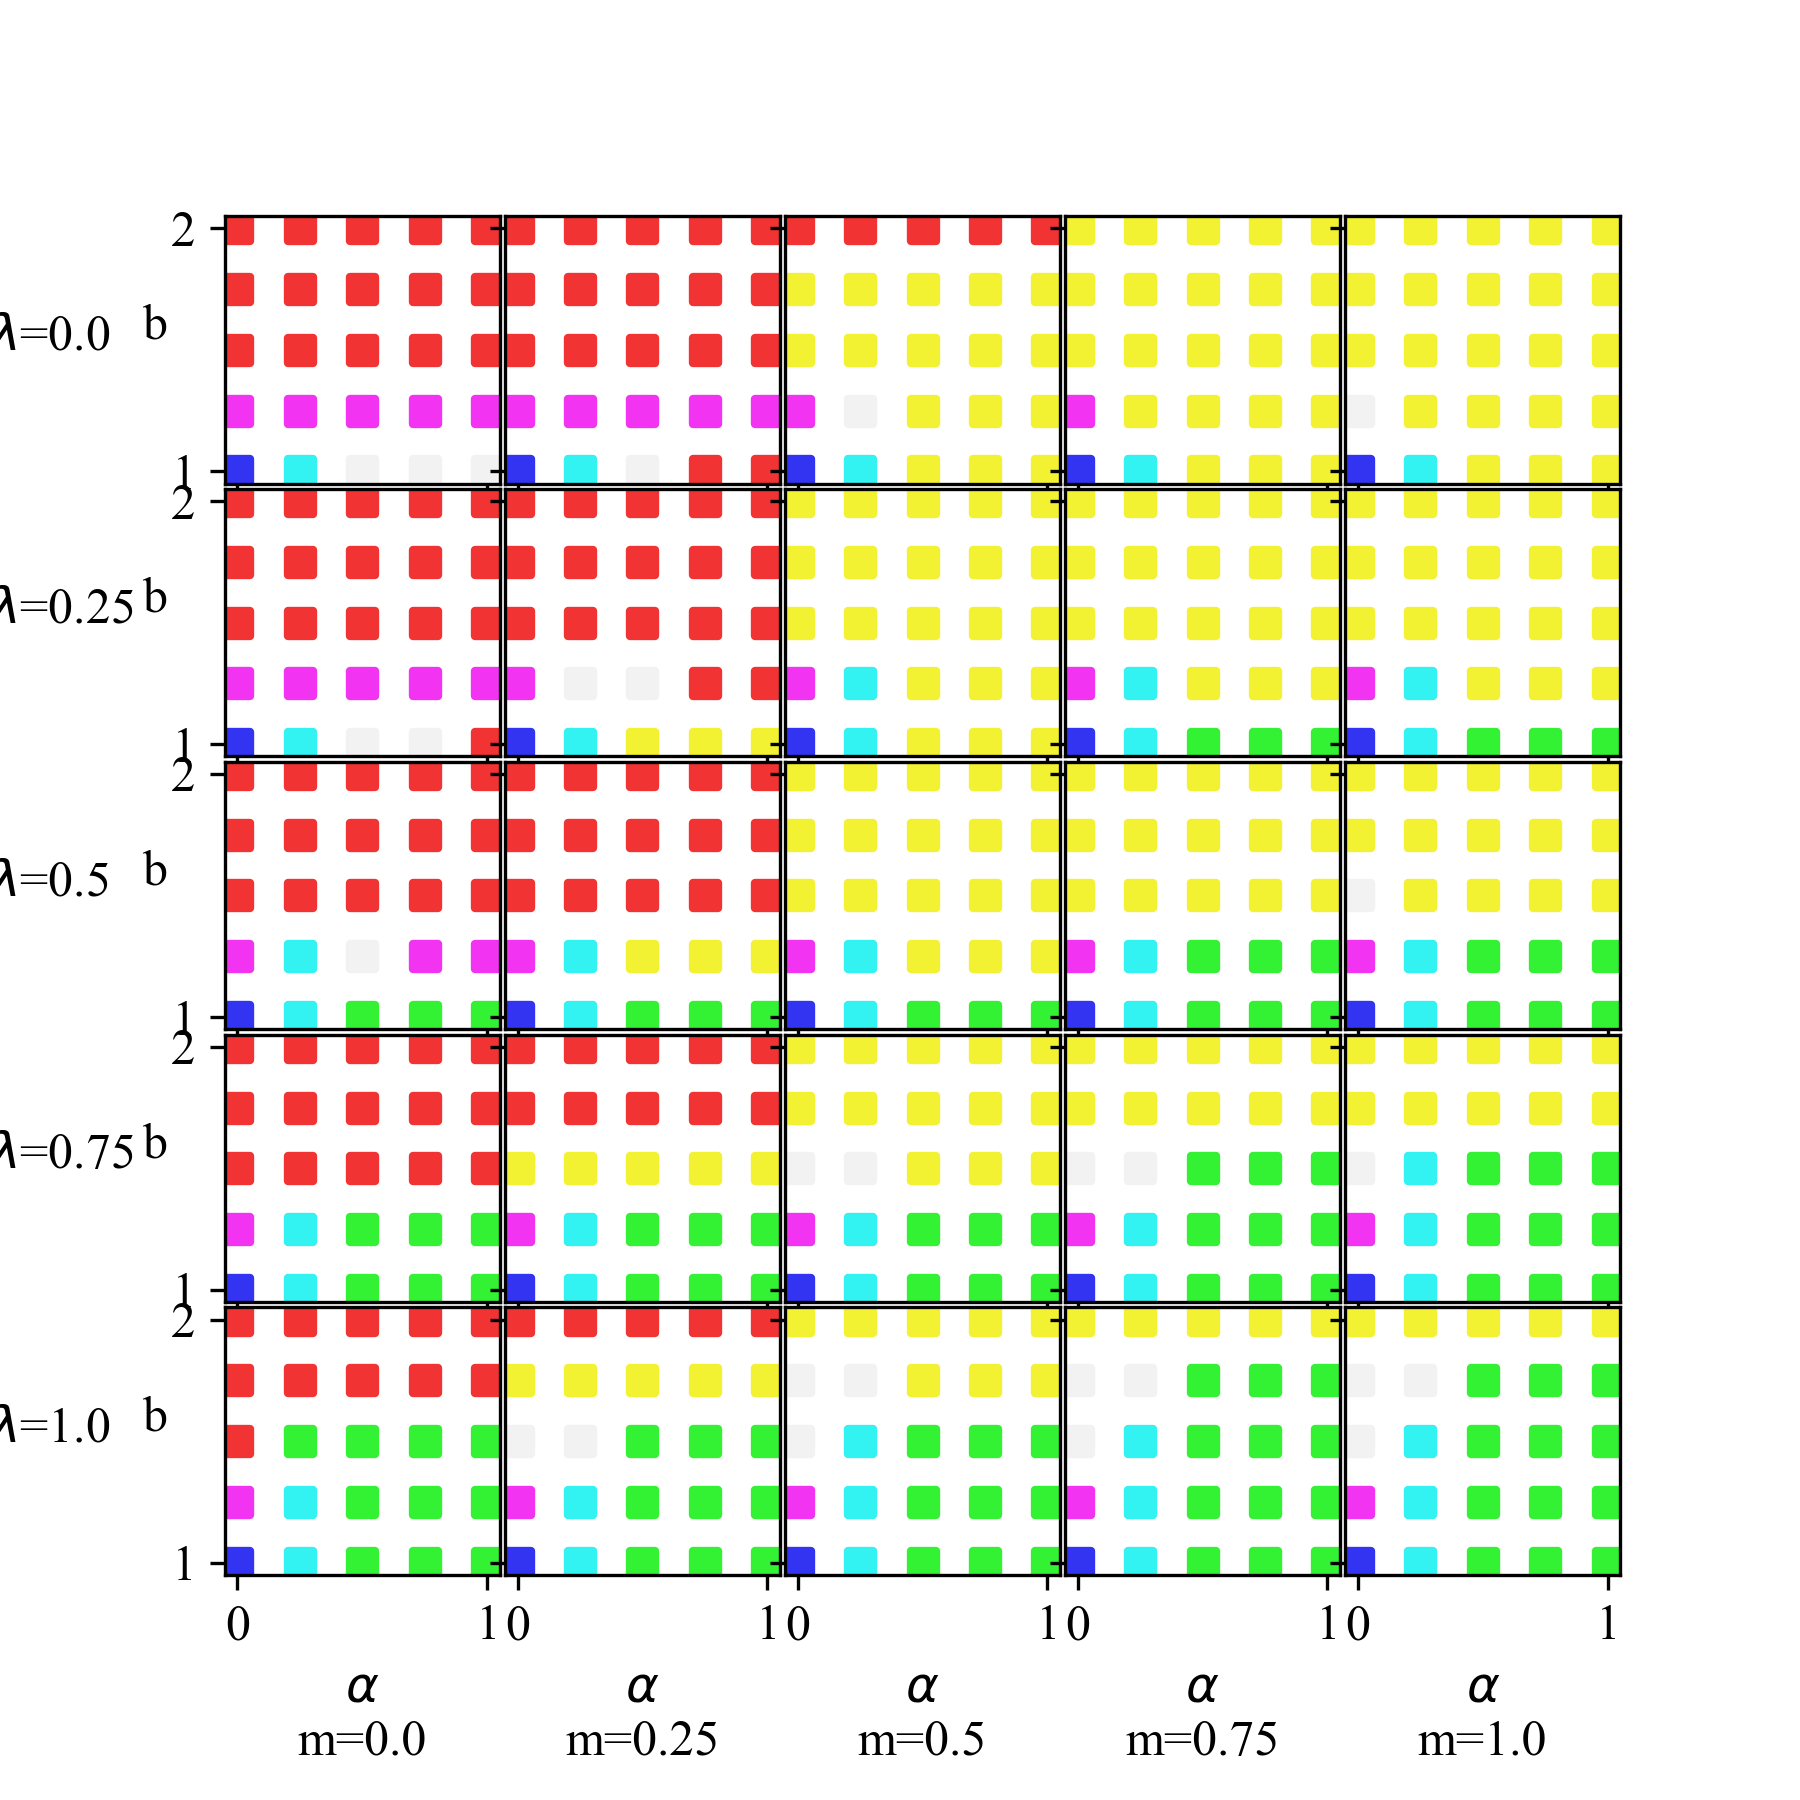
\includegraphics[width=\textwidth]{D025R050.png}
    \caption{When $\delta = 0.25$ and $\rho = 0.5$}
    \label{fig:d25r050}
\end{figure}

\begin{figure}[h]
    \centering
    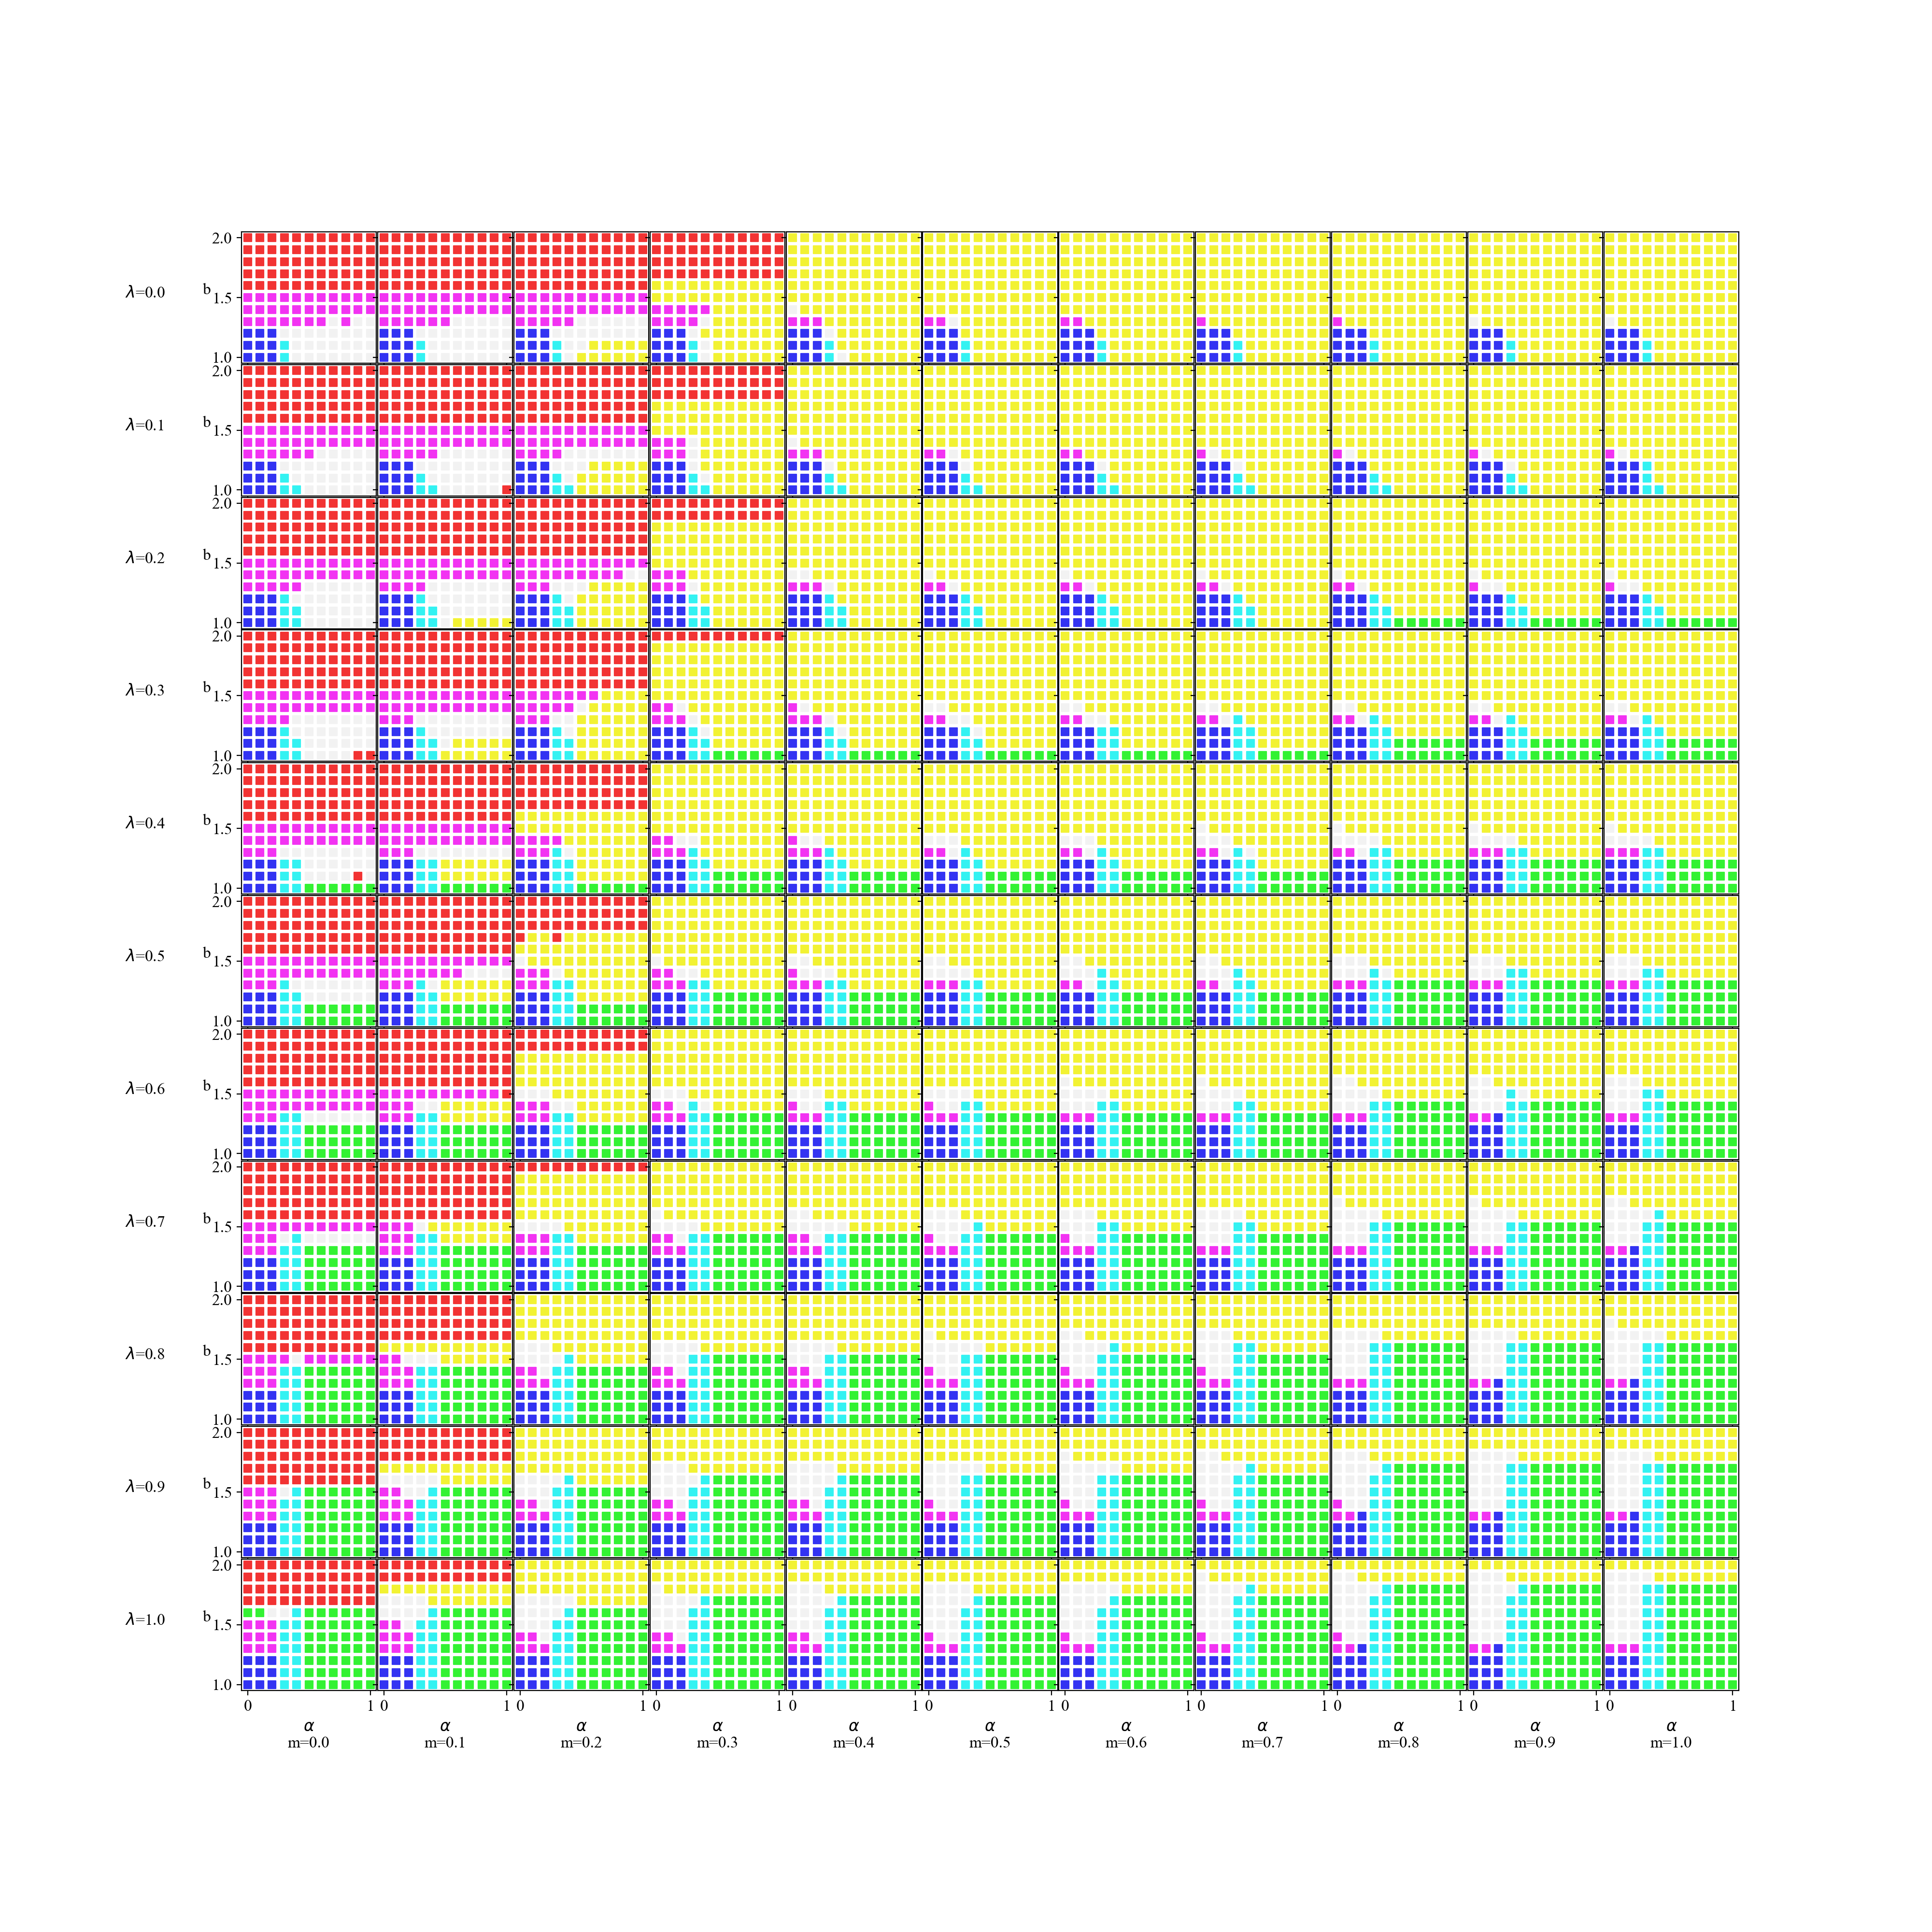
\includegraphics[width=\textwidth]{Four_D010R050.png}
    \caption{When $\delta = 0.1, \rho = 0.5$}
    \label{fig:d01r05}
\end{figure}

For the whole 25 figures in one, here is the $\delta \times \rho$ Fig.\ref{fig:all025}.

\begin{figure}
    \centering
    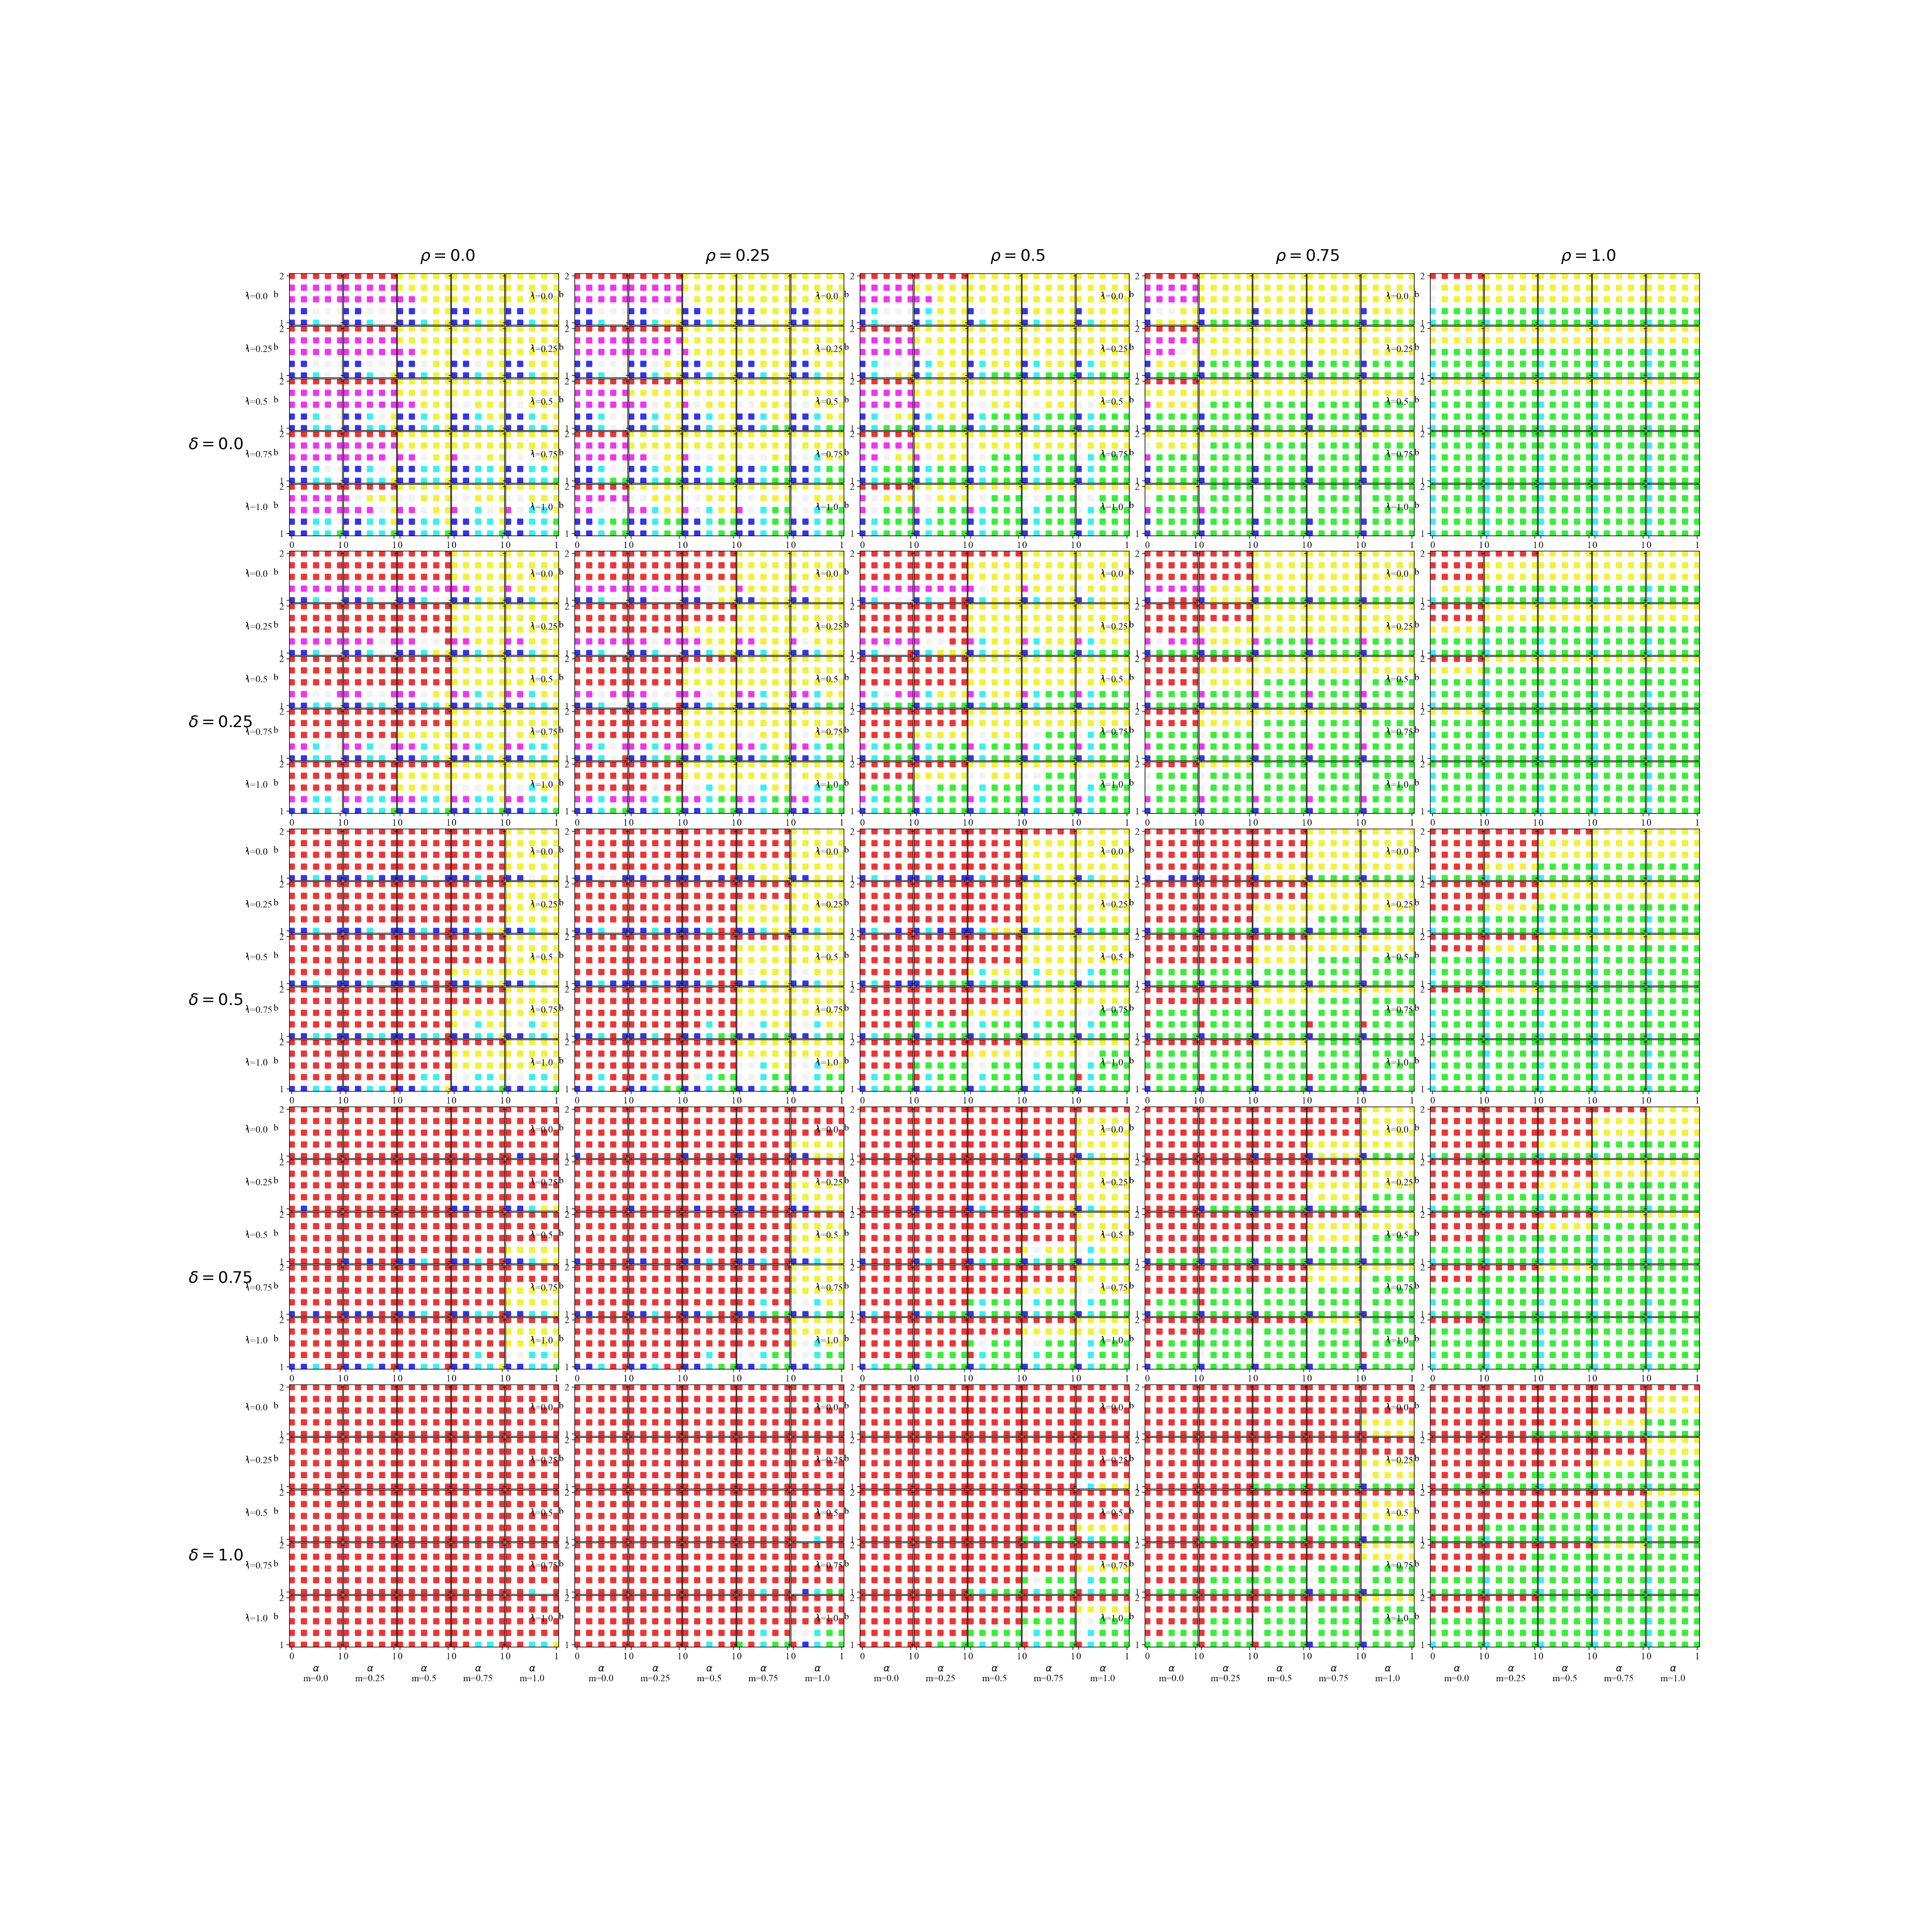
\includegraphics[width=\textwidth]{All_gap025.png}
    \caption{All 15625 simulations with gap $0.25$}
    \label{fig:all025}
\end{figure}

\section{Feb 8th}

\begin{figure}[t!] % "[t!]" placement specifier just for this example
\begin{subfigure}{0.48\textwidth}
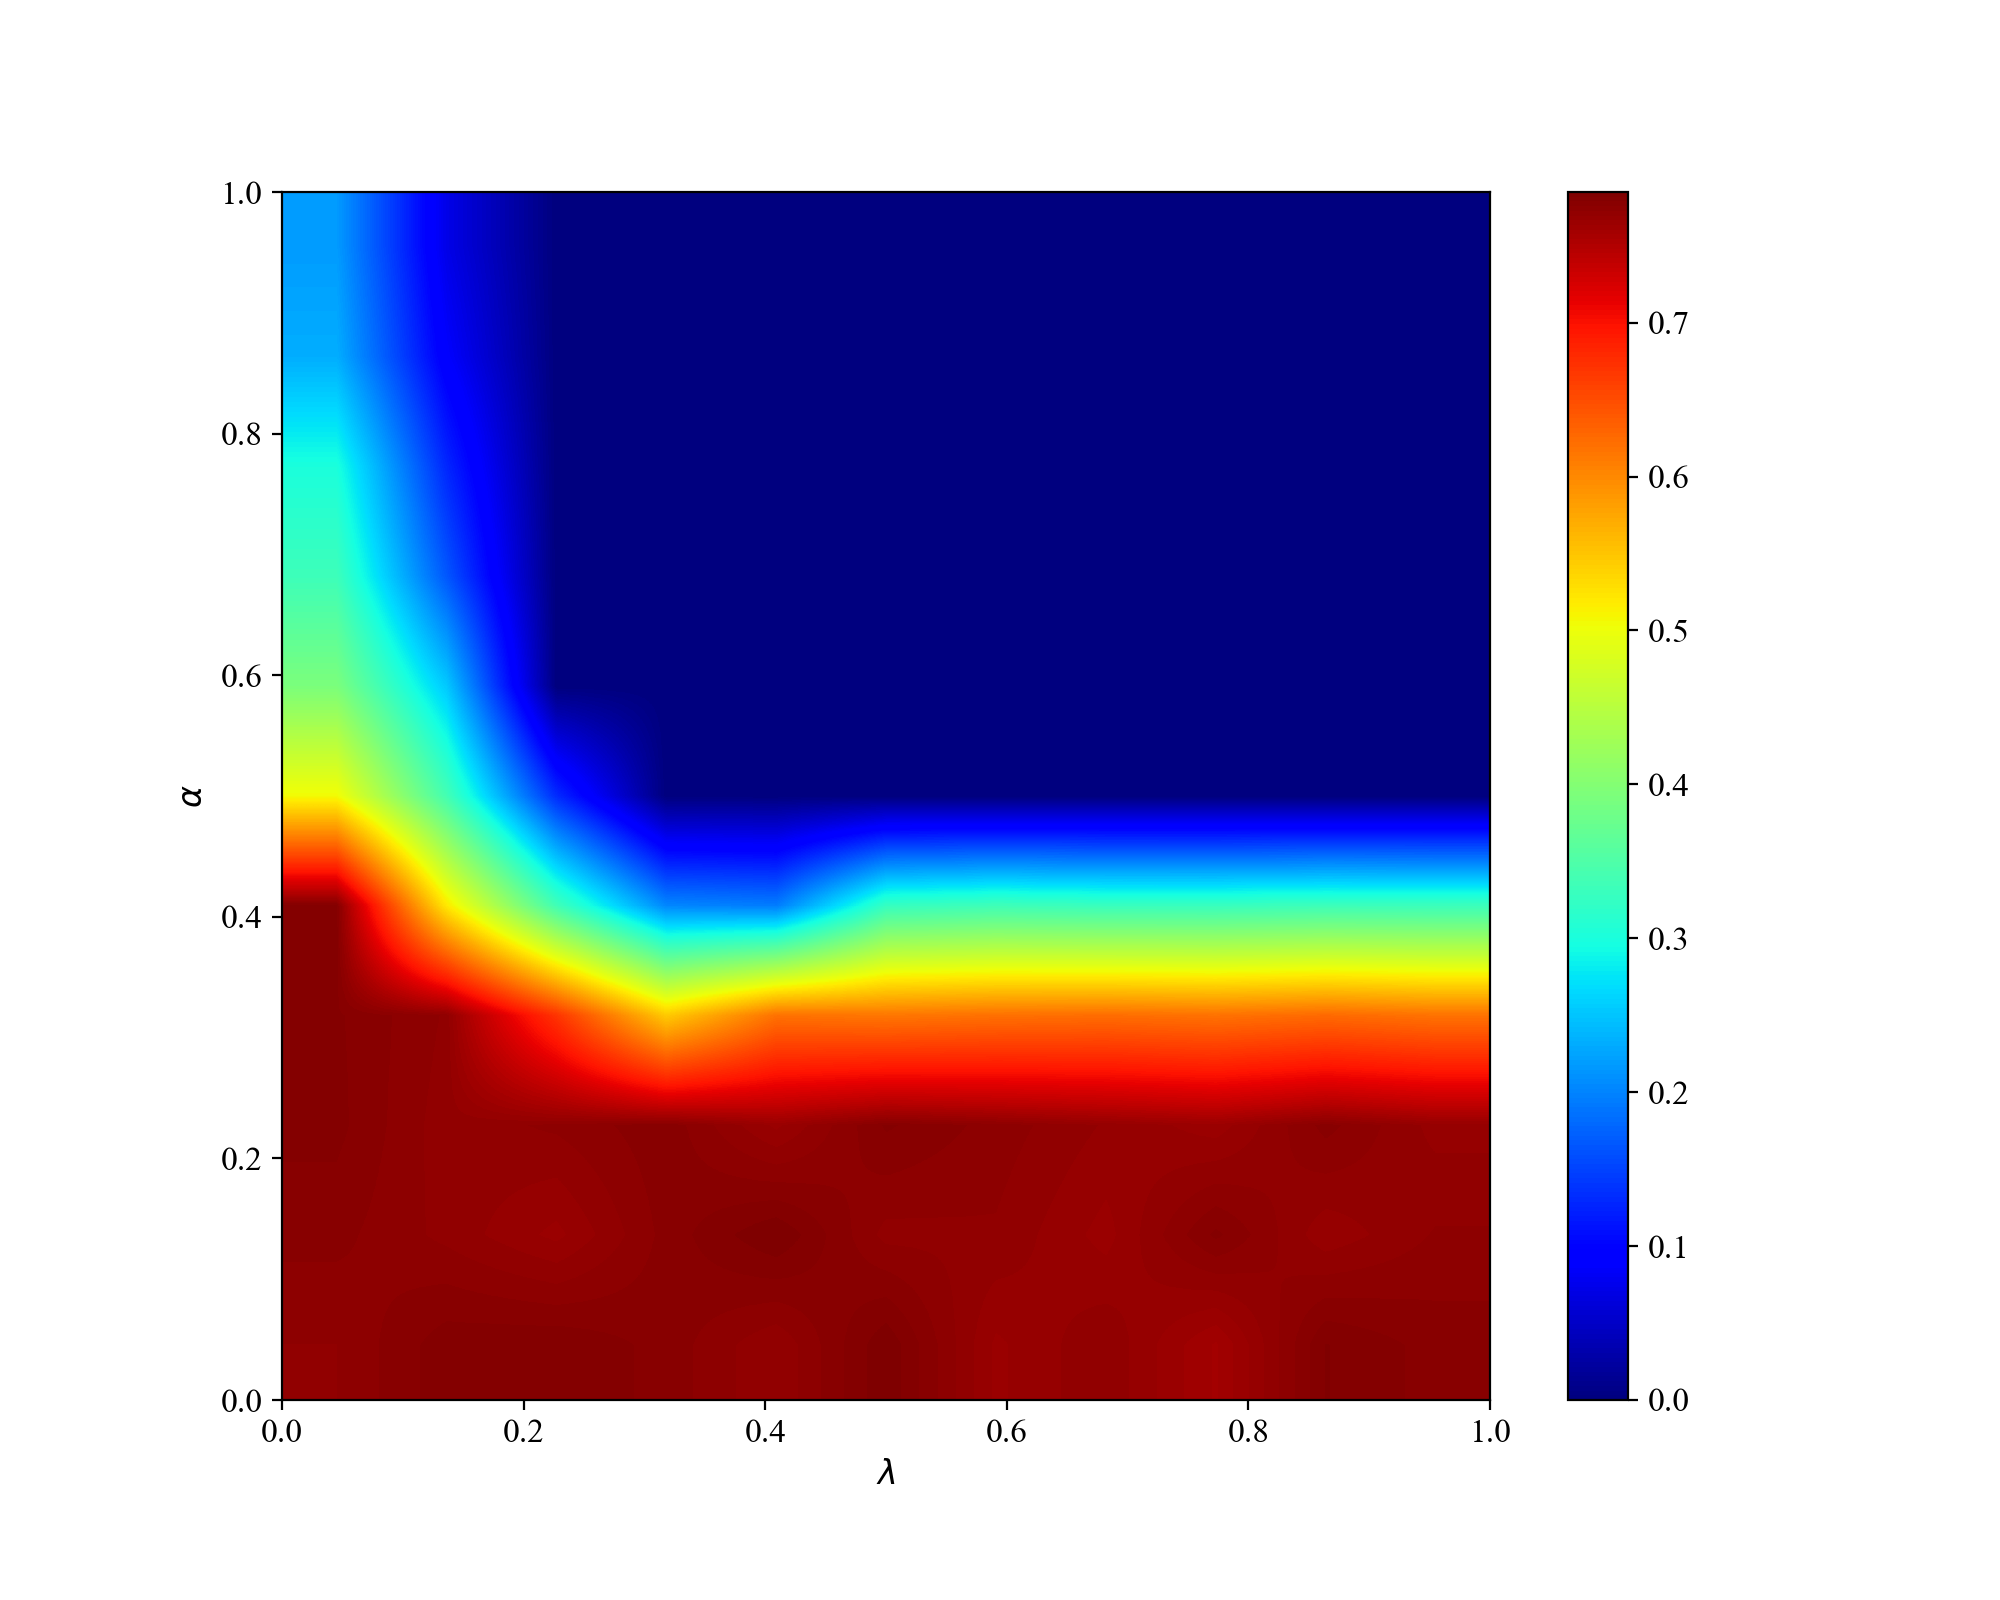
\includegraphics[width=\linewidth]{b013_1.png}
\caption{First subfigure} \label{fig:a}
\end{subfigure}\hspace*{\fill}
\begin{subfigure}{0.48\textwidth}
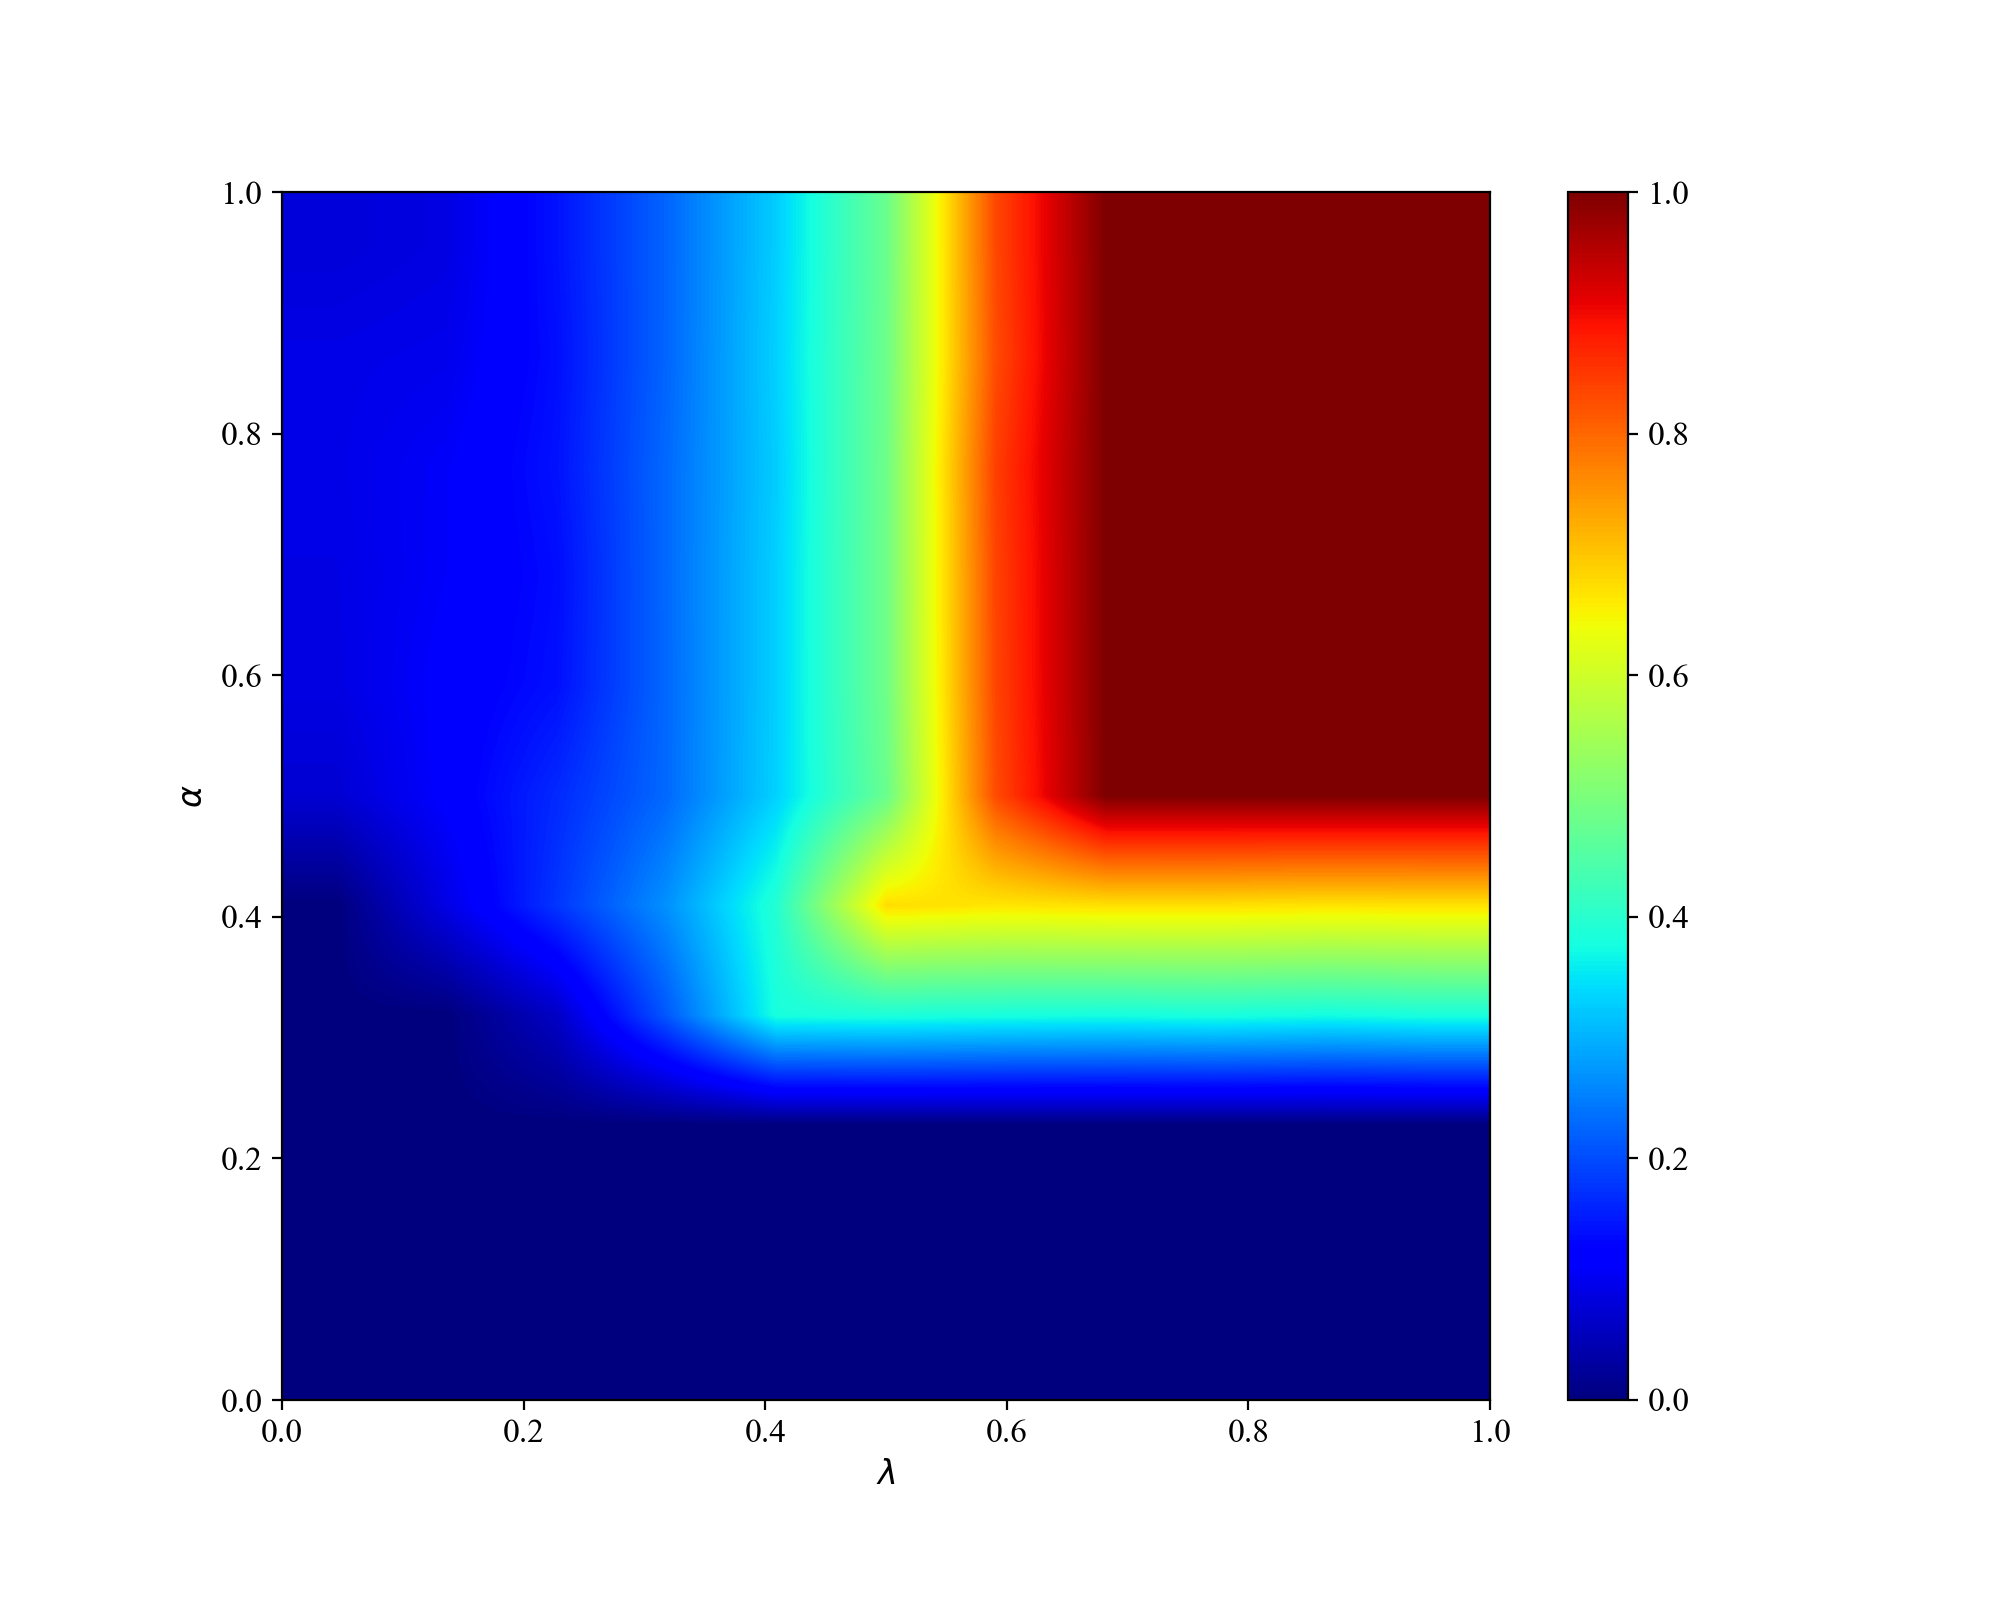
\includegraphics[width=\linewidth]{b013_2.png}
\caption{Second subfigure} \label{fig:b}
\end{subfigure}\hspace*{\fill}
\begin{subfigure}{0.48\textwidth}
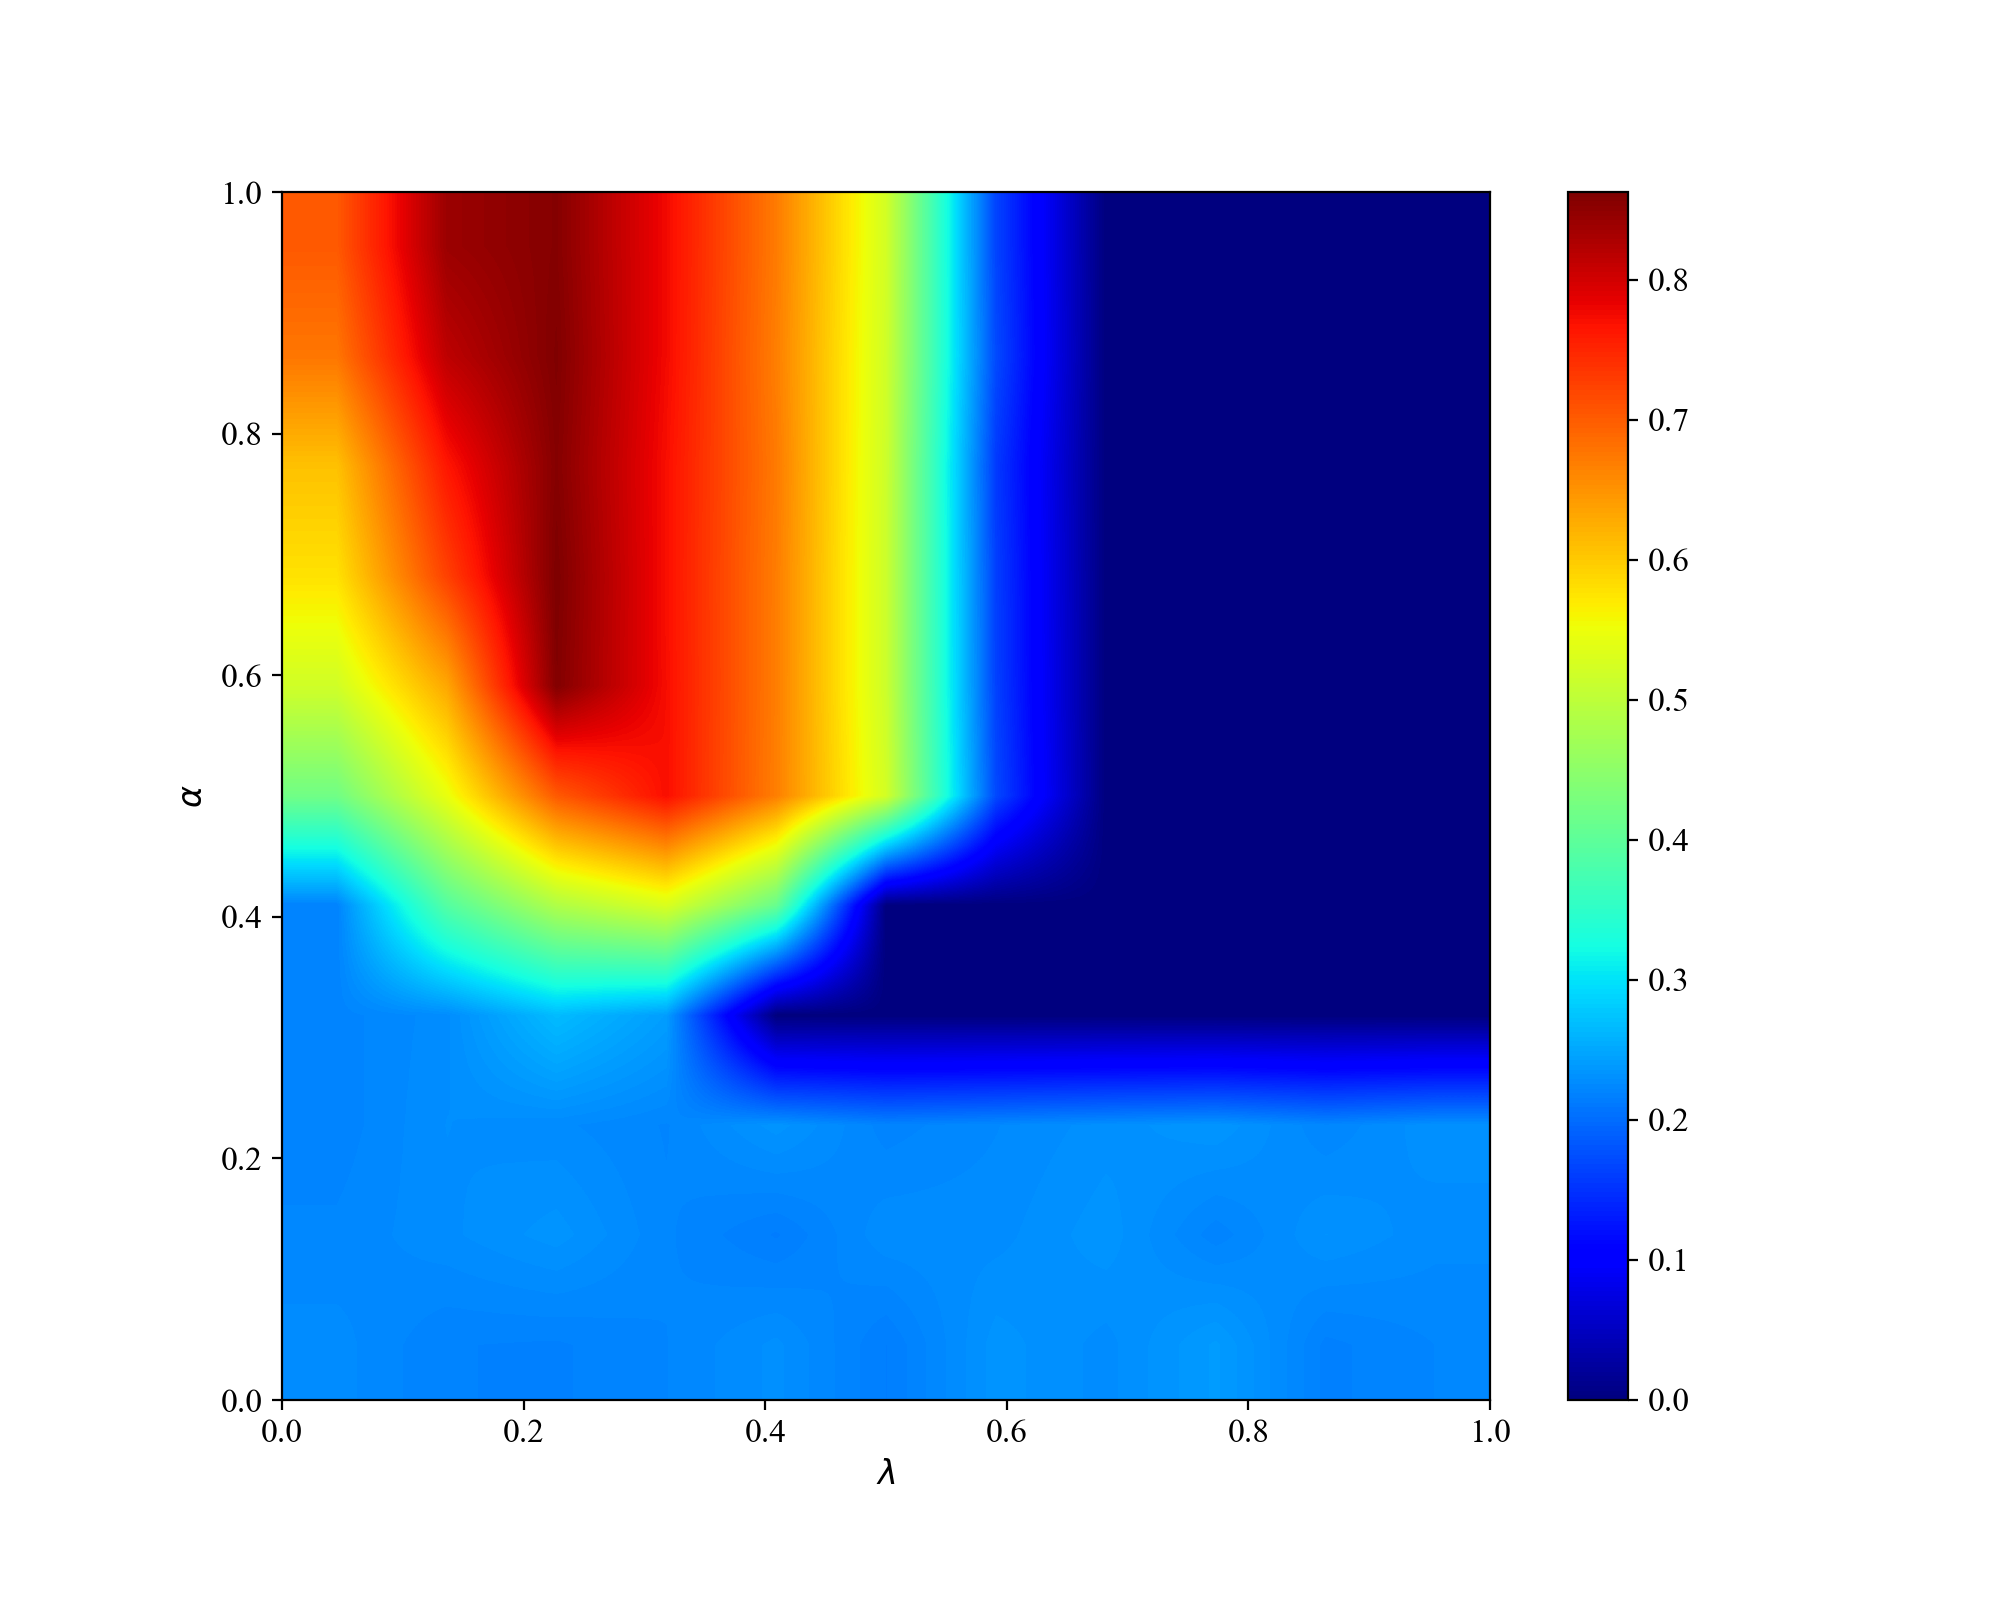
\includegraphics[width=\linewidth]{b013_0.png}
\caption{Third subfigure} \label{fig:c}
\end{subfigure}\hspace*{\fill}

\medskip

\begin{subfigure}{0.48\textwidth}
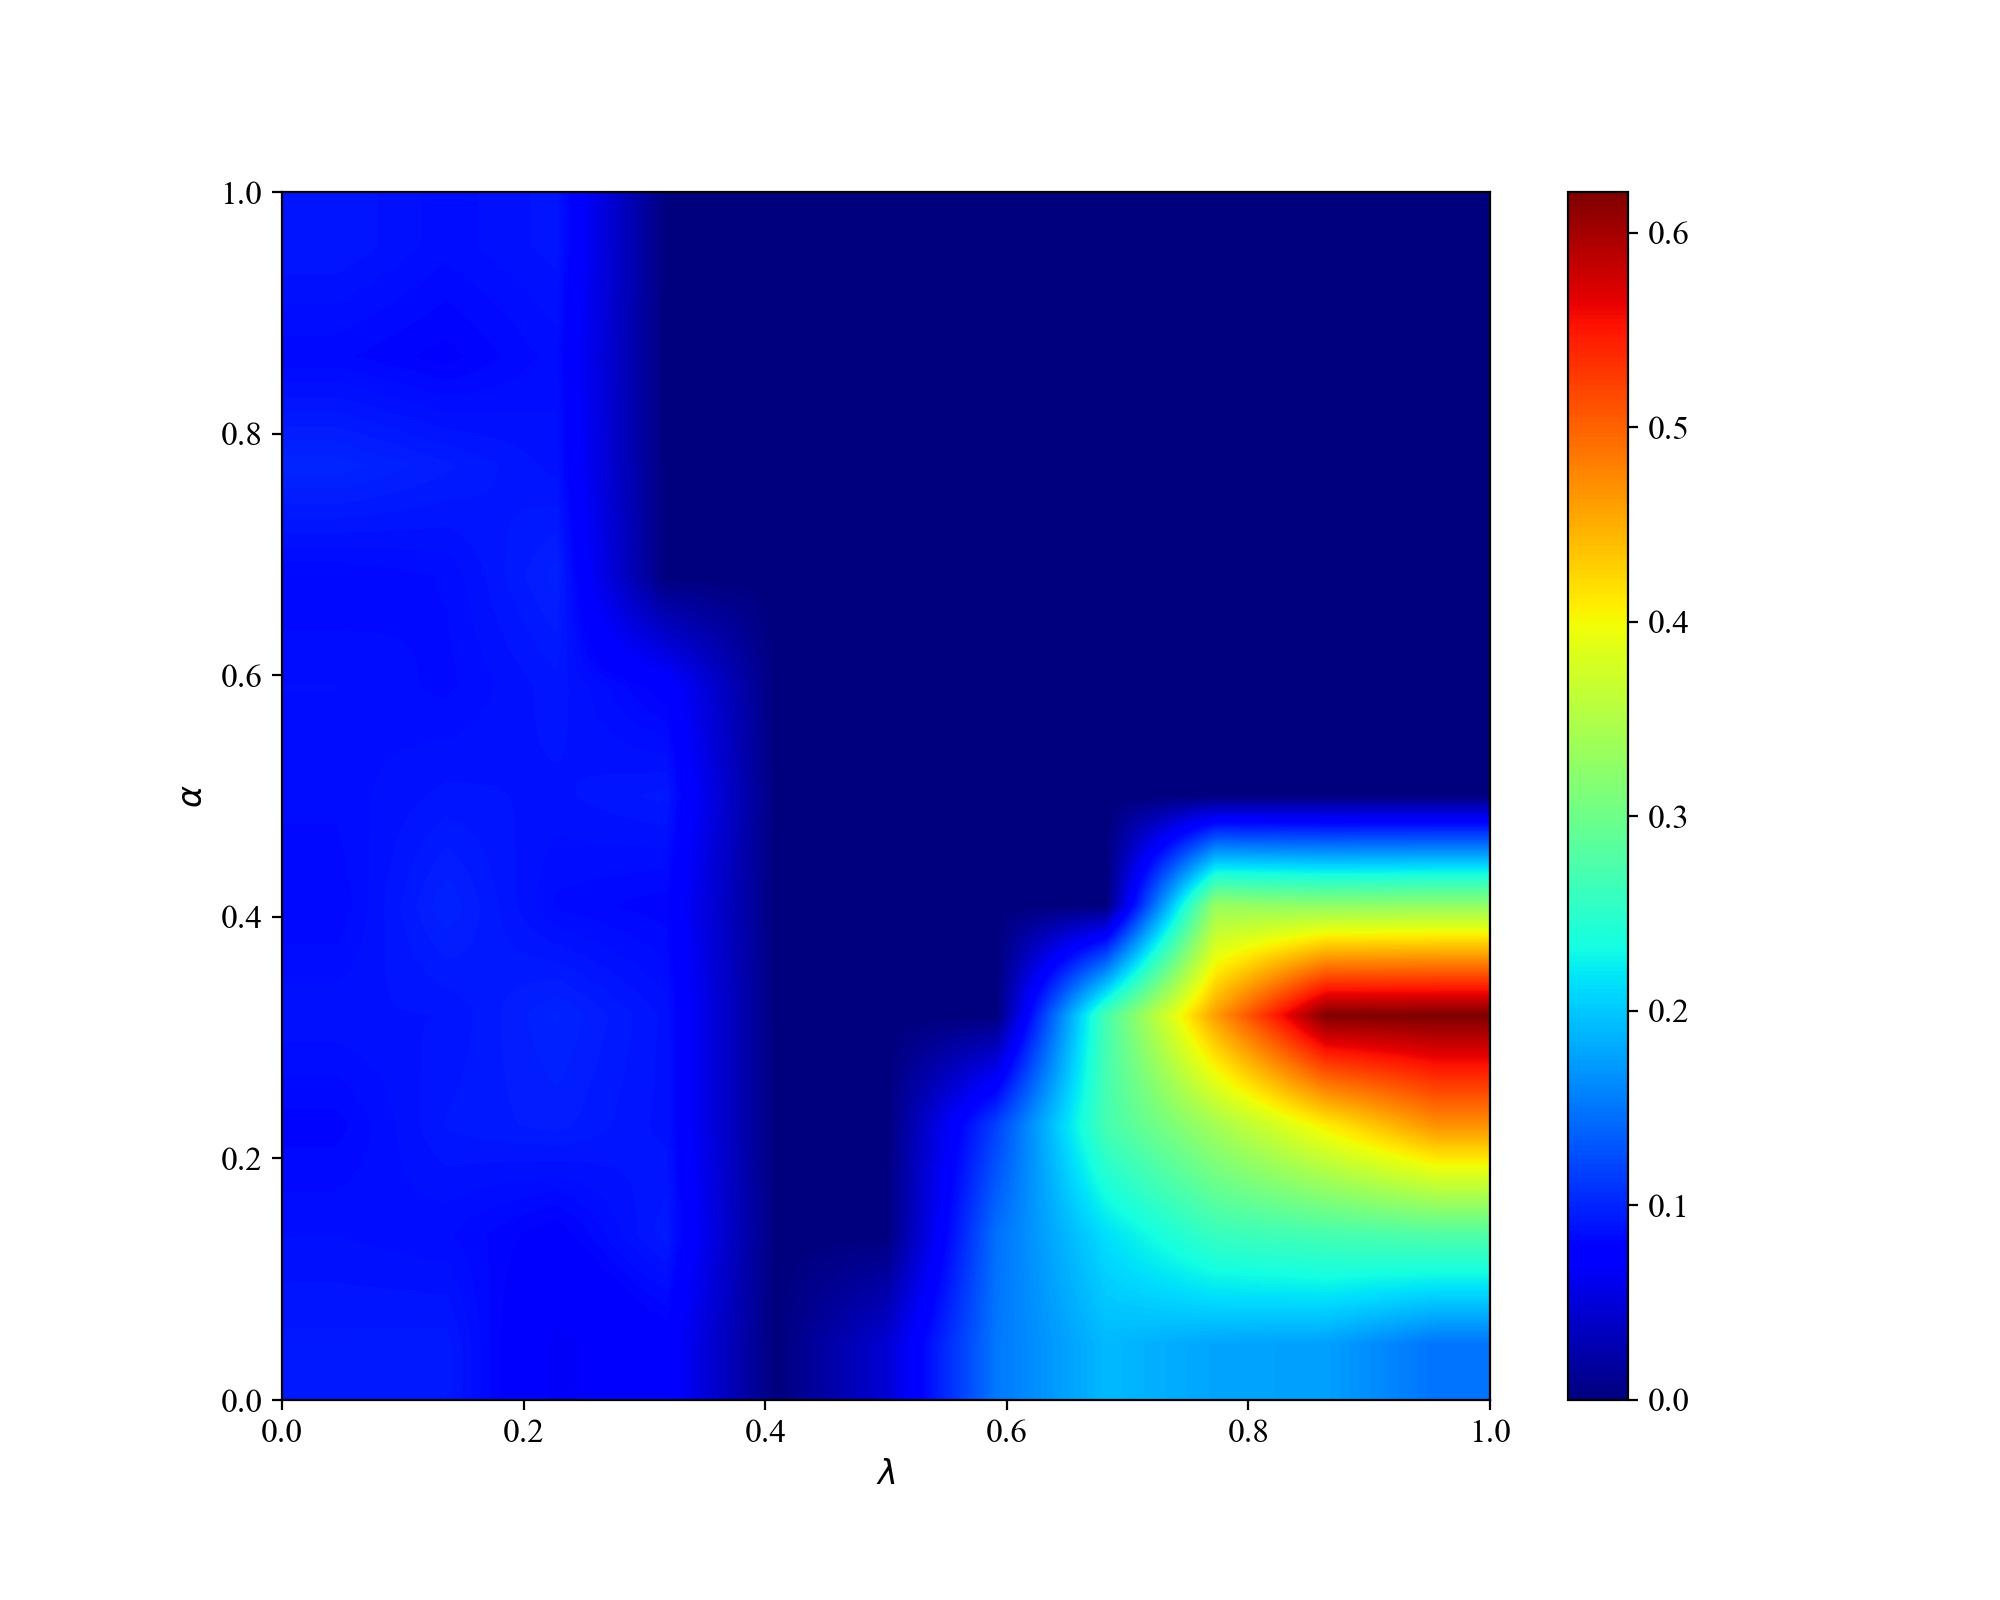
\includegraphics[width=\linewidth]{b015_1.png}
\caption{Fourth subfigure} \label{fig:d}
\end{subfigure}
\begin{subfigure}{0.48\textwidth}
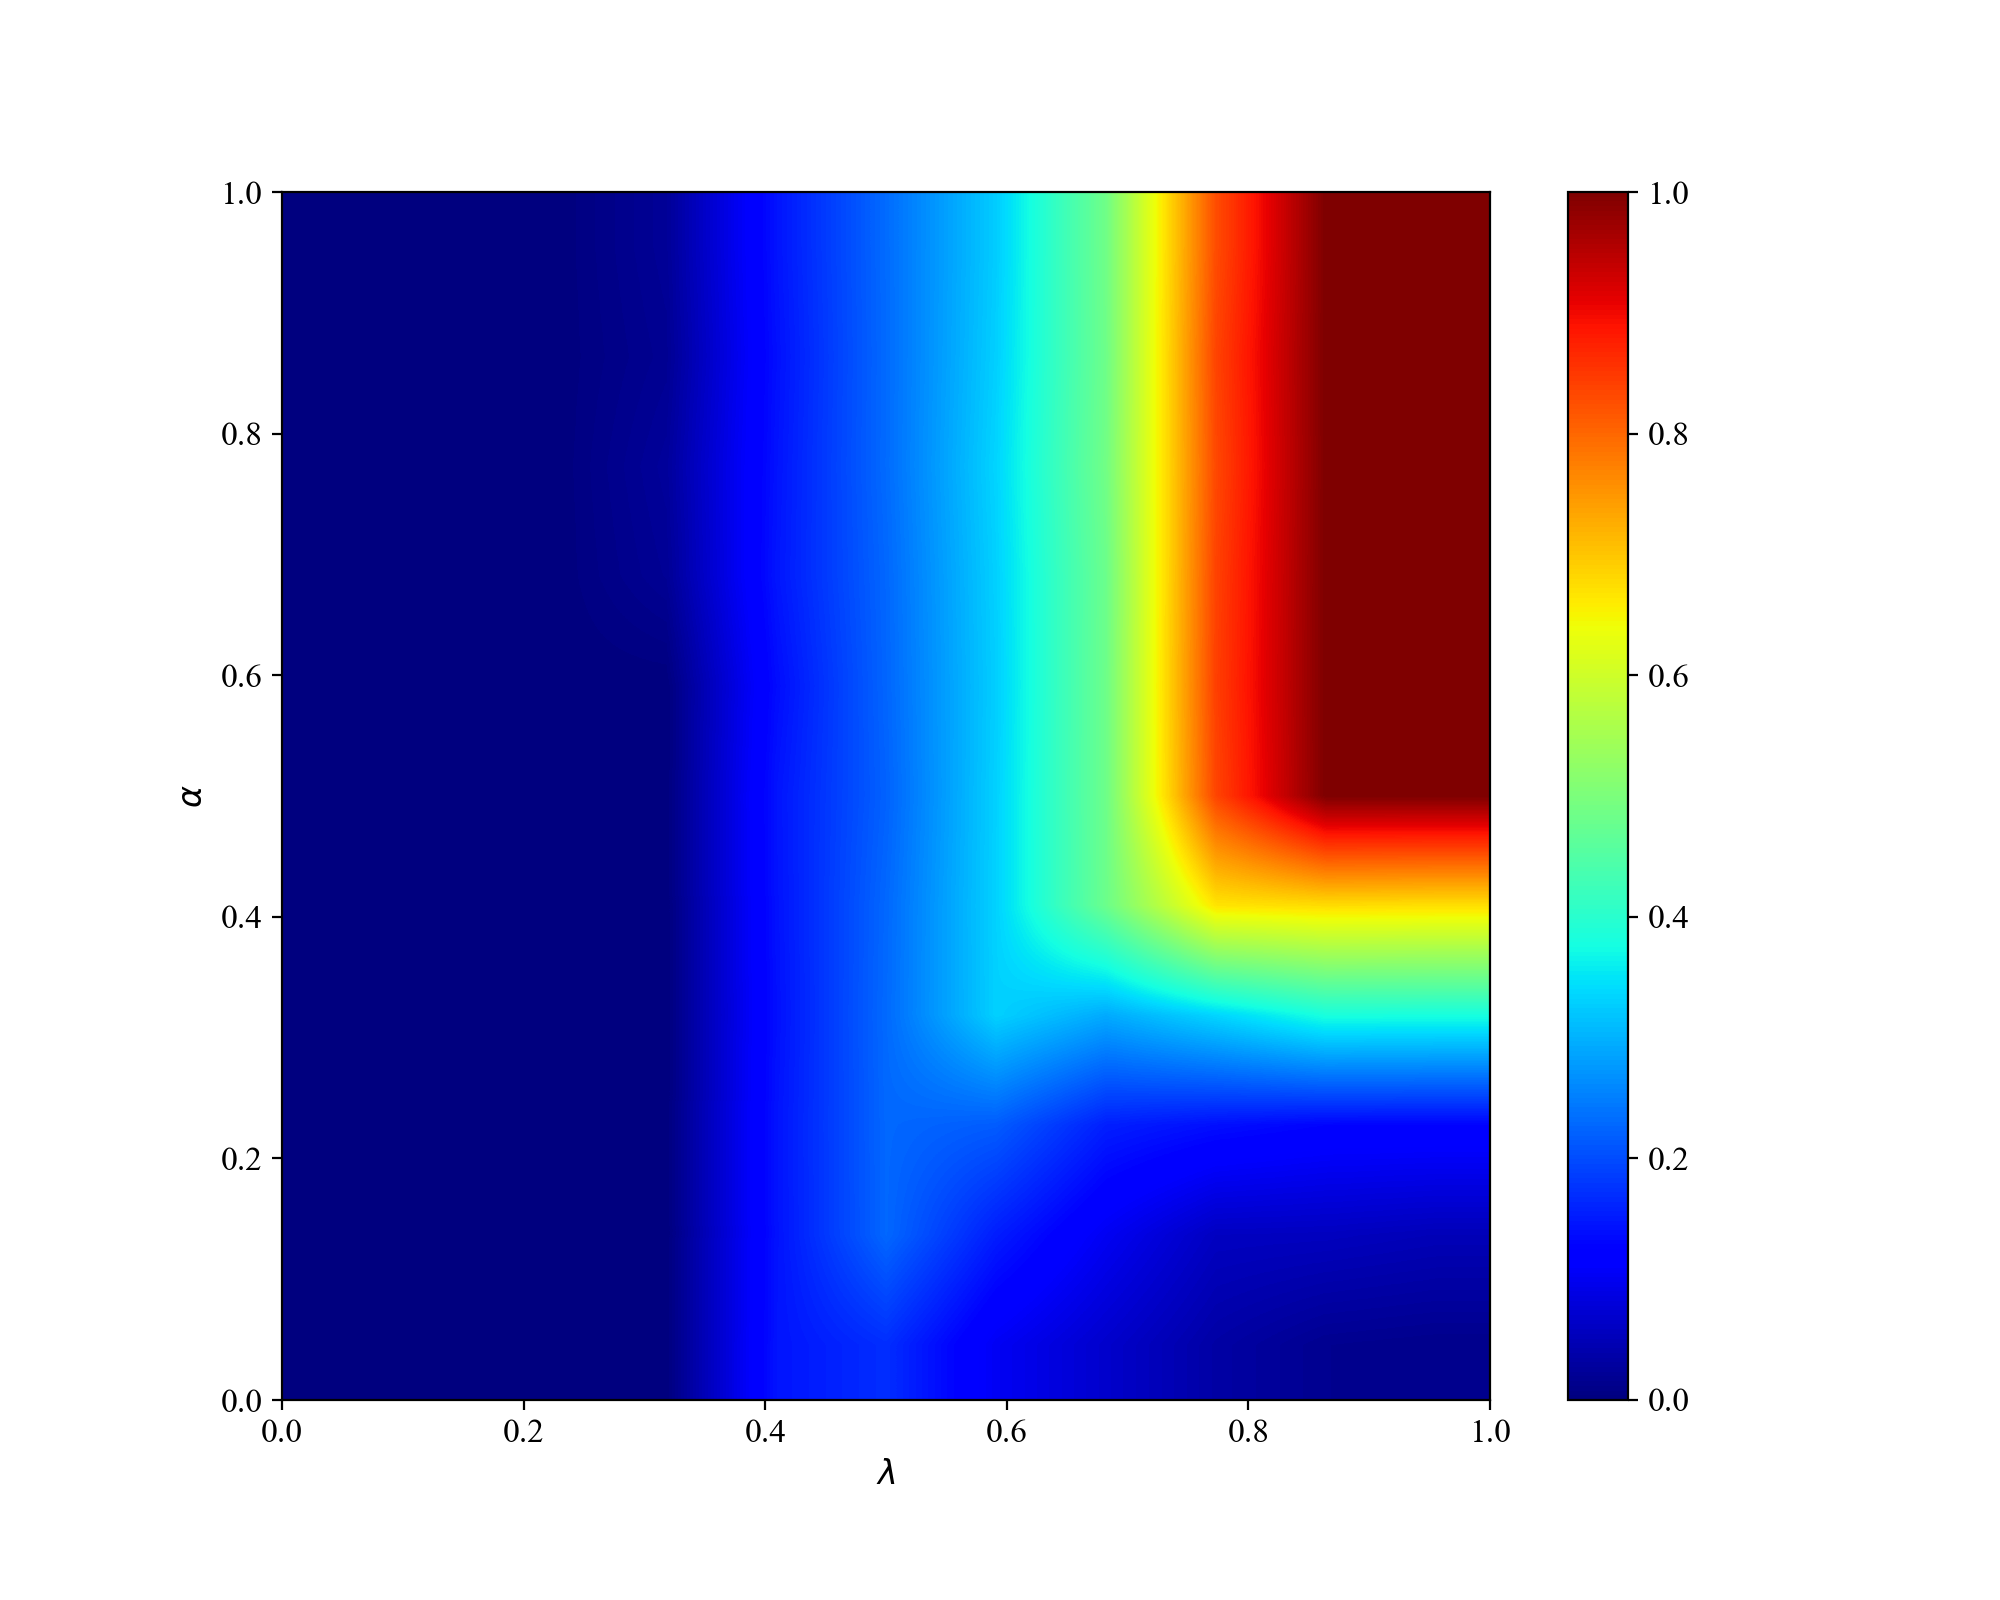
\includegraphics[width=\linewidth]{b015_2.png}
\caption{Fifth subfigure} \label{fig:e}
\end{subfigure}\hspace*{\fill}
\begin{subfigure}{0.48\textwidth}
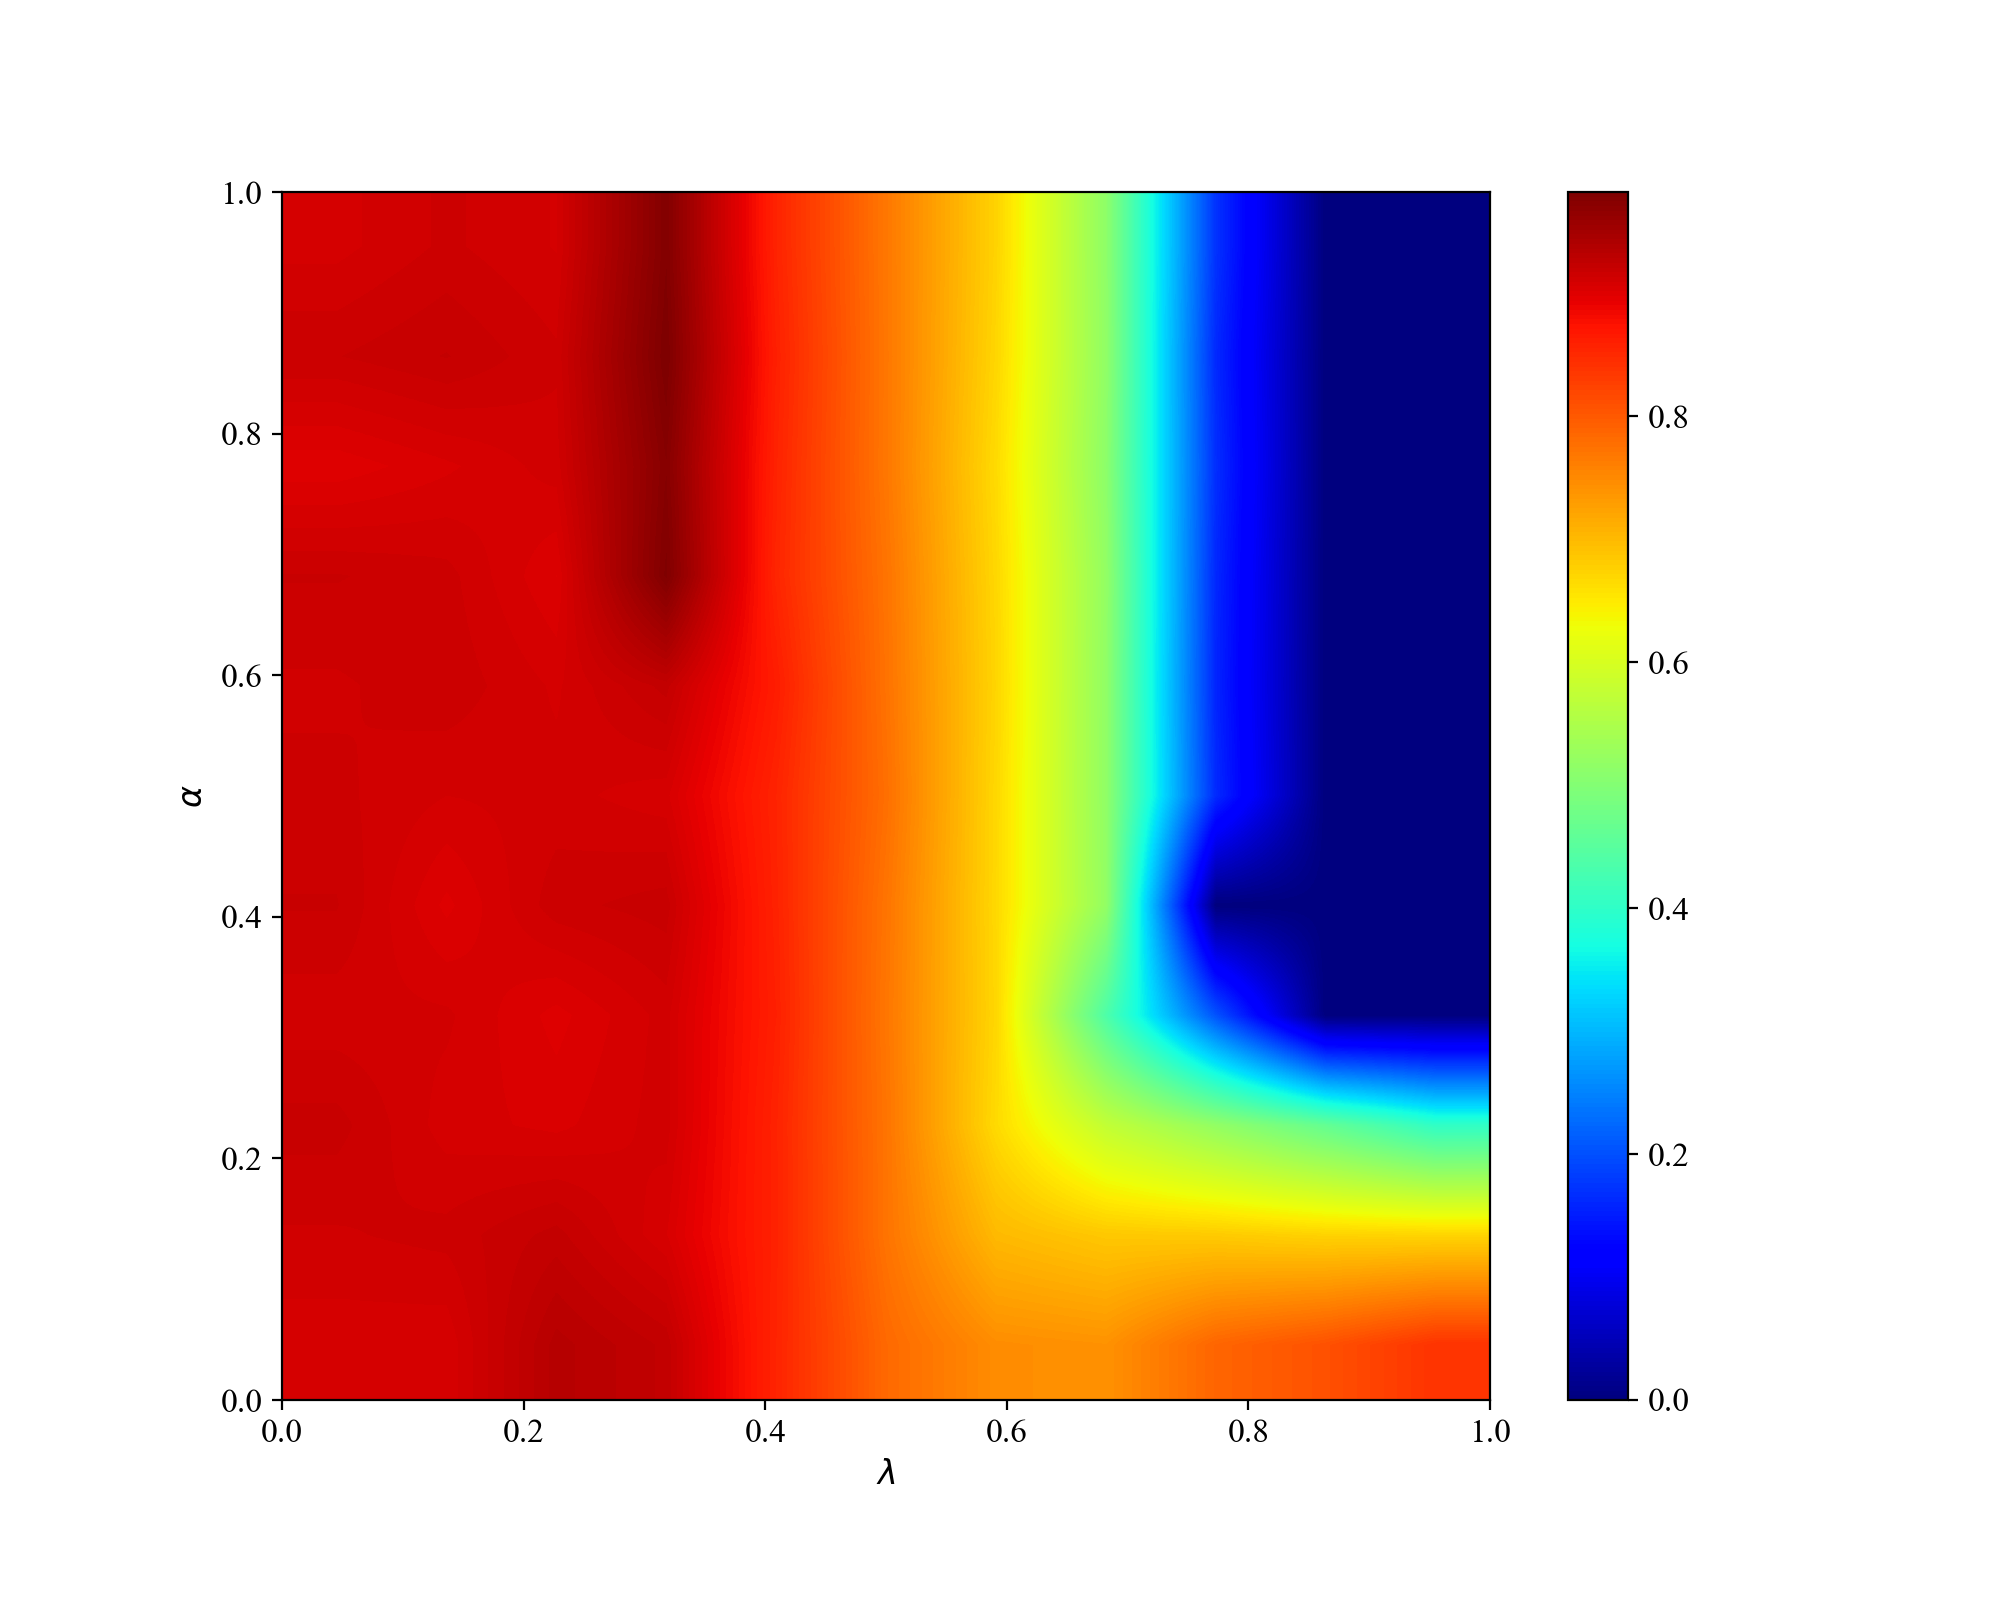
\includegraphics[width=\linewidth]{b015_0.png}
\caption{Sixth subfigure} \label{fig:f}
\end{subfigure}

\caption{My complicated figure} \label{fig:1}
\end{figure}

\clearpage

\section{Feb 13th}
\begin{figure}[h]
    \centering
    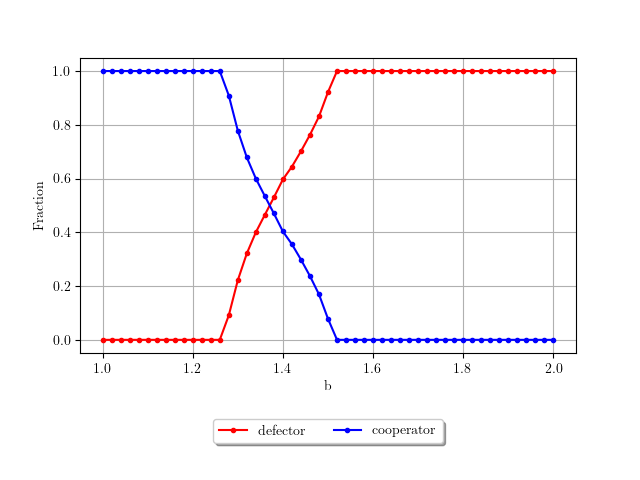
\includegraphics[width=\textwidth]{Only_two_b.png}
    \caption{Only two: When $\delta = 0.1, \rho = 0.5$}
    \label{fig:onlytwo}
\end{figure}




 
\end{document}
